%&bericht

%%%%%%%%%%%%%%%%%%%%%%%%%%%%%%%%%%%%%%%%%%%%%%%%%%%%%%%%%%%%%%%%%%%%%%%%%%%%%%%
%% Descr:       Vorlage für Berichte der DHBW-Karlsruhe
%% Author:      Prof. Dr. Jürgen Vollmer, juergen.vollmer@dhbw-karlsruhe.de
%% $Id: bericht.tex,v 1.25 2020/03/13 15:07:45 vollmer Exp $
%%  -*- coding: utf-8 -*-
%%%%%%%%%%%%%%%%%%%%%%%%%%%%%%%%%%%%%%%%%%%%%%%%%%%%%%%%%%%%%%%%%%%%%%%%%%%%%%%

\documentclass[
   ngerman          % neue deutsche Rechtschreibung
  ,a4paper          % Papiergrösse
%  ,twoside          % Zweiseitiger Druck (rechts/links)
%  ,10pt             % Schriftgrösse
%  ,11pt
 ,12pt
  ,pdftex
%  ,disable         % Todo-Markierungen auschalten
]{report}

%\usepackage[fontsize=13pt]{scrextend}
\usepackage{setspace}

% Bitte die Codierung Ihrer Dateien auswählen:
% \usepackage[latin1]{inputenc}    % Für UNIX mit ISO-LATIN-codierten Dateien
% \usepackage[applemac]{inputenc}  % Für Apple Mac
% \usepackage[ansinew]{inputenc}   % Für Microsoft Windows
\usepackage[utf8]{inputenc}   % UTF-8 codierte Dateien
\usepackage{tabularx}     
                                   % Dieses Dokument ist unter Unix erstellt, daher
                                   % wird diese Input-Codierung benutzt.
\usepackage{bericht}
%% ACHTUNG, wenn man eine eigene Formatdatei (bericht.fmt) benutzt, werden Änderungen an bericht.sty
%% erst wirksam, wenn die Format-Datei neu erzeugt wurde!!!
%% Genauer alle Änderungen, die textuell vor der nächsten Zeile ".... endofdump...." stehen
%% werden erst wirksam, wenn die Formatdatei neu erzeugt wurde
\csname endofdump\endcsname

%%%%%%%%%%%%%%%%%%%%%%%%%%%%%%%%%%%%%%%%%%%%%%%%%%%%%%%%%%%%%%%%%%%%%%%%%%%%%%%
%% Angaben zur Arbeit
%%%%%%%%%%%%%%%%%%%%%%%%%%%%%%%%%%%%%%%%%%%%%%%%%%%%%%%%%%%%%%%%%%%%%%%%%%%%%%%

\newcommand{\Autor}{Burak Özkan und Daniel Schomburg}
\newcommand{\MatrikelNummer}{9015631 und 6218975}
\newcommand{\Kursbezeichnung}{Tinf20B3}

% Falls es kein Firmenlogo gibt:
%  \newcommand{\FirmenLogoDeckblatt}{}

%\newcommand{\BetreuerFirma}{Titel Vorname Nachname}
\newcommand{\BetreuerDHBW}{Danie Lindner}

%%%%%%%%%%%%%%%%%%%%%%%%%%%%%%%%%%%%%%%%%%%%%%%%%%%%%%%%%%%%%%%%%%%%%%%%%%%%%%%%%%%%%

% Wird auf dem Deckblatt und in der Erklärung benutzt:
\newcommand{\Was}{Studienarbeit}

%%%%%%%%%%%%%%%%%%%%%%%%%%%%%%%%%%%%%%%%%%%%%%%%%%%%%%%%%%%%%%%%%%%%%%%%%%%%%%%%%%%%%

\newcommand{\Titel}{DHBW-Star App}
\newcommand{\AbgabeDatum}{22. Mai 2023}

%\newcommand{\Dauer}{ Wochen}

% \newcommand{\Abschluss}{Bachelor of Engineering}
\newcommand{\Abschluss}{Bachelor of Science}

\newcommand{\Studiengang}{Informatik / Informationstechnik}

\hypersetup{%%
  pdfauthor={\Autor},
  pdftitle={\Titel},
  pdfsubject={\Was}
}

%%%%%%%%%%%%%%%%%%%%%%%%%%%%%%%%%%%%%%%%%%%%%%%%%%%%%%%%%%%%%%%%%%%%%%%%%%%%%%%

% Wenn \includeonly{..} benutzt wird, werden nur diese Kaptitel ausgegeben.
\includeonly{
  abk
 ,kapitel1
 ,kapitel2
 ,kapitel3
 ,kapitel4
 ,kapitel5
 ,kapitel6
 ,changelog
}

%%%%%%%%%%%%%%%%%%%%%%%%%%%%%%%%%%%%%%%%%%%%%%%%%%%%%%%%%%%%%%%%%%%%%%%%%%%%%%%

% Benutzt man das "biblatex"-Paket, dann muß das hier stehen:
% siehe auch die mit BIBLATEX markierten Zeilen in bericht.sty
\bibliography{bericht}

\begin{document}

%%%%%%%%%%%%%%%%%%%%%%%%%%%%%%%%%%%%%%%%%%%%%%%%%%%%%%%%%%%%%%%%%%%%%%%%%%%%%%%

\begin{titlepage}
\begin{center}
\vspace*{-2cm}
\hfill
\includegraphics[width=3cm]{dhbw-logo}\\[2cm]
{\Huge \Titel}\\[1cm]
{\Huge\scshape \Was}\\[1cm]
{\large für die Prüfung zum}\\[0.5cm]
{\Large \Abschluss}\\[0.5cm]
{\large des Studienganges \Studiengang}\\[0.5cm]
{\large an der}\\[0.5cm]
{\large Dualen Hochschule Baden-Württemberg Karlsruhe}\\[0.5cm]
{\large von}\\[0.5cm]
{\large\bfseries \Autor}\\[1cm]
{\large Abgabedatum \AbgabeDatum}
\vfill
\end{center}
\begin{tabular}{l@{\hspace{2cm}}l}
%Bearbeitungszeitraum	        & \Dauer 			\\
Matrikelnummer	                & \MatrikelNummer	\\
Kurs			         		& \Kursbezeichnung	\\
Gutachter der Studienakademie	& \BetreuerDHBW	  	\\
\end{tabular}
\end{titlepage}

%%%%%%%%%%%%%%%%%%%%%%%%%%%%%%%%%%%%%%%%%%%%%%%%%%%%%%%%%%%%%%%%%%%%%%%%%%%%%%%

%%%%%%%%%%%%%%%%%%%%%%%%%%%%%%%%%%%%%%%%%%%%%%%%%%%%%%%%%%%%%%%%%%%%%%%%%%%%%%%
%% Descr:       Vorlage für Berichte der DHBW-Karlsruhe, Erklärung
%% Author:      Prof. Dr. Jürgen Vollmer, vollmer@dhbw-karlsruhe.de
%% $Id: erklaerung.tex,v 1.11 2020/03/13 14:24:42 vollmer Exp $
%% -*- coding: utf-8 -*-
%%%%%%%%%%%%%%%%%%%%%%%%%%%%%%%%%%%%%%%%%%%%%%%%%%%%%%%%%%%%%%%%%%%%%%%%%%%%%%%

% In Bachelorarbeiten muss eine schriftliche Erklärung abgegeben werden.
% Hierin bestätigen die Studierenden, dass die Bachelorarbeit, etc.
% selbständig verfasst und sämtliche Quellen und Hilfsmittel angegeben sind. Diese Erklärung
% bildet das zweite Blatt der Arbeit. Der Text dieser Erklärung muss auf einer separaten Seite
% wie unten angegeben lauten.

\newpage
\thispagestyle{empty}
\begin{framed}
\begin{center}
\Large\bfseries Erklärung
\end{center}
\medskip
\noindent
% siehe §5(3) der \enquote{Studien- und Prüfungsordnung DHBW Technik} vom 29.\,9.\,2017 und Anhang 1.1.13
Ich versichere hiermit, dass ich meine \Was mit dem Thema:
\enquote{\Titel}
selbstständig verfasst und keine anderen als die angegebenen Quellen und Hilfsmittel benutzt habe. Ich versichere zudem, dass die eingereichte elektronische Fassung mit der gedruckten Fassung übereinstimmt. \newline
\vspace{2cm}
\linebreak
\noindent
\underline{\hspace{4cm}}\hfill\underline{\hspace{6cm}}\\
Ort~~~~~Datum\hfill Unterschrift\hspace{4cm}
\\\\\\
\underline{\hspace{4cm}}\hfill\underline{\hspace{6cm}}\\
Ort~~~~~Datum\hfill Unterschrift\hspace{4cm}
\end{framed}

%\vfill
%\emph{Sofern vom Dualen Partner ein Sperrvermerk gewünscht wird, ist folgende Formulierung
%zu verwenden:}
%\begin{framed}
%\begin{center}
%\Large\bfseries Sperrvermerk
%\end{center}
%\medskip
%\noindent
%Der Inhalt dieser Arbeit darf weder als Ganzes noch in Auszügen Personen
%außerhalb des Prüfungsprozesses und des Evaluationsverfahrens zugänglich gemacht
%werden, sofern keine anderslautende Genehmigung vom Dualen Partner vorliegt.
%\end{framed}

%%%%%%%%%%%%%%%%%%%%%%%%%%%%%%%%%%%%%%%%%%%%%%%%%%%%%%%%%%%%%%%%%%%%%%%%%%%%%%%
\endinput
%%%%%%%%%%%%%%%%%%%%%%%%%%%%%%%%%%%%%%%%%%%%%%%%%%%%%%%%%%%%%%%%%%%%%%%%%%%%%%%


%%%%%%%%%%%%%%%%%%%%%%%%%%%%%%%%%%%%%%%%%%%%%%%%%%%%%%%%%%%%%%%%%%%%%%%%%%%%%%%

\begin{abstract}
Fortschritte in der Digitalisierung läuteten eine neue Ära in der Hochschulbildung ein
und veränderten die Art und Weise, wie Studierende ihre Bildungserfahrungen
gestalten. In dieser Situation ist es wichtig, dass Studierende jederzeit Zugriff auf
Informationen zu Lehrveranstaltungen, Prüfungen, Veranstaltungen etc. haben. Die
Gemeinsame Staatliche Hochschule Baden-Württemberg (DHBW) Karlsruhe ist eine
der führenden deutschen Hochschulen mit dem Ziel, Studierende umfassend zu
informieren. Diese Studienarbeit beschreibt die Entwicklung einer App, die Probleme
mit Informationen der DHBW Karlsruhe identifiziert und die Zentralisierung aller
Informationen auf der App.

Es wurden umfangreiche Recherchen durchgeführt, um aktuelle Fragestellungen zu
identifizieren, die in den von der DHBW Karlsruhe zur Durchführung des Projekts
bereitgestellten Informationen enthalten sind. Zusätzlich wurden die App-
Anforderungen definiert und ein Prototyp entwickelt. Um die Benutzerfreundlichkeit
und Funktionalität der App zu evaluieren, wurde eine Studentenbefragung
durchgeführt.

Die App bietet Studenten eine Reihe von Funktionen, darunter Zugriff auf alle
relevanten Informationen, einfache Navigation durch verschiedene Kurse und die
Möglichkeit, Feedback zu geben und Probleme zu melden. Feedback wird in Echtzeit
an die zuständige Abteilung weitergeleitet, um eine schnellstmögliche Lösung zu
ermöglichen. Durch die zentrale Sammlung aller Informationen in der App haben die
Studierenden schnellen und einfachen Zugriff auf alle relevanten Informationen.
Die Implementierung der App brachte viele Vorteile, darunter eine verbesserte
Benutzerfreundlichkeit und den Zugriff auf alle relevanten Informationen an einem
Ort. Die Schüler haben Zugang zu einer Vielzahl von Informationen, damit sie ihre
Bildungserfahrung besser gestalten können. Eine Feedback-Funktion ermöglicht es
den Schülern, Probleme zu melden und Verbesserungen vorzuschlagen, um die
bereitgestellten Informationen zu verbessern.

Eine App zur Erkennung von Problemen mit Informationen der DHBW Karlsruhe und
zur Zentralisierung aller Informationen in der App ist ein wertvolles Instrument zur
Verbesserung des Informationsangebots der Hochschule. Die App ist einfach zu
bedienen und bietet Schülern umfassende Informationen, die ihnen helfen, ihre
Bildungserfahrung zu gestalten. Darüber hinaus bietet die Feedback-Funktion den
Studierenden eine Plattform, um ihr Feedback und ihre Vorschläge zur Verbesserung
des Informationsangebots der DHBW Karlsruhe zu teilen.

\end{abstract}

\newpage
\tableofcontents           % Inhaltsverzeichnis hier ausgeben
\listoffigures             % Liste der Abbildungen
\listoftables              % Liste der Tabellen
\lstlistoflistings         % Liste der Listings
\listofequations           % Liste der Formeln

% Jetzt kommt der "eigentliche" Text
%%%%%%%%%%%%%%%%%%%%%%%%%%%%%%%%%%%%%%%%%%%%%%%%%%%%%%%%%%%%%%%%%%%%%%%%%%%%%%
%% Descr:       Vorlage für Berichte der DHBW-Karlsruhe, Datei mit Abkürzungen
%% Author:      Prof. Dr. Jürgen Vollmer, vollmer@dhbw-karlsruhe.de
%% $Id: abk.tex,v 1.4 2017/10/06 14:02:03 vollmer Exp $
%% -*- coding: utf-8 -*-
%%%%%%%%%%%%%%%%%%%%%%%%%%%%%%%%%%%%%%%%%%%%%%%%%%%%%%%%%%%%%%%%%%%%%%%%%%%%%%%

\chapter*{Abkürzungsverzeichnis}                   % chapter*{..} -->   keine Nummer, kein "Kapitel"
						         % Nicht ins Inhaltsverzeichnis
% \addcontentsline{toc}{chapter}{Akürzungsverzeichnis}   % Damit das doch ins Inhaltsverzeichnis kommt

% Hier werden die Abkürzungen definiert
\begin{acronym}[DHBW]
  % \acro{Name}{Darstellung der Abkürzung}{Langform der Abkürzung}
 \acro{Abk}[Abk.]{Abkürzung}

 % Folgendes benutzen, wenn der Plural einer Abk. benöigt wird
 % \newacroplural{Name}{Darstellung der Abkürzung}{Langform der Abkürzung}
 \newacroplural{Abk}[Abk-en]{Abkürzungen}

 \acro{H2O}[\ensuremath{H_2O}]{Di-Hydrogen-Monoxid}

 % Wenn neicht benutzt, erscheint diese Abk. nicht in der Liste
 \acro{NUA}{Not Used Acronym}
\end{acronym}
              % Abkürzungsverzeichnis
\begin{onehalfspace}
\chapter{Einleitung}
Die fortschreitende Digitalisierung hat in den letzten Jahren weitreichende Veränderungen in der Hochschulwelt mit sich gebracht. Immer mehr Bildungseinrichtungen nutzen digitale Informationskanäle, um Studierende, Mitarbeiter und andere Interessengruppen über aktuelle Ereignisse, Veranstaltungen und wichtige Informationen auf dem Laufenden zu halten \cite{aachenerzeitung2022}. Die Duale Hochschule Baden-Württemberg (DHBW) Karlsruhe bildet da keine Ausnahme.

Mit langjähriger Erfahrung als Hochschule für angewandte Wissenschaften hat die DHBW Karlsruhe vielfältige Informationen geschaffen, um den Bedürfnissen ihrer Nutzer gerecht zu werden \cite{degruyter2021}. Bei der Bereitstellung von Informationen für eine große Anzahl von Benutzern können jedoch verschiedene Probleme auftreten.

Die Digitalisierung der Hochschulbildung stellt nicht nur akademische Inhalte in digitaler Form bereit, sondern eröffnet auch neue pädagogische Möglichkeiten zur Wissens- und Kompetenzvermittlung. \cite{hochschulforumdigitalisierung} Es ist daher Aufgabe der Hochschulleitung sowie der Konzeption konkreter Lehrveranstaltungen und Lernmaterialien, diese digitalen Möglichkeiten zu nutzen und weiterzuentwickeln \cite{springerlink2023}. 

Bei der Umsetzung dieser digitalen Transformation können jedoch auch Hindernisse auftreten, wie beispielsweise unsere natürliche Widerstandsfähigkeit gegenüber schnellen Veränderungen \cite{degruyter2021_2}. Dennoch müssen diese Herausforderungen angegangen werden, wenn wir die Chancen der Digitalisierung maximieren und die Hochschulbildung zukunftssicher machen wollen.
\\\\
\emph{Für die Rechtschreib- und Grammatikprüfung dieser Studienarbeit wird\\ https://www.scribbr.de/rechtschreibpruefung/ verwendet} 

\section{Hintergrund und Kontext}
Die Duale Hochschule Baden-Württemberg (DHBW) Karlsruhe ist eine der größten Hochschulen für angewandte Wissenschaften in Deutschland. Mit über 8.000 Studierenden und mehr als 1.000 Mitarbeitern bietet die DHBW Karlsruhe ein breites Spektrum an Studiengängen in verschiedenen Fachbereichen an. Um den Anforderungen ihrer Nutzer gerecht zu werden, hat die DHBW Karlsruhe in den letzten Jahren eine Vielzahl von Informationsangeboten entwickelt, wie z.B. die Website, die Intranet-Plattform und verschiedene soziale Medien.

Aktuelle Informationsangebote werden derzeit über verschiedene Plattformen angeboten. Der Stundenplan kann beispielsweise über das Rapla-System eingesehen werden, Informationen zur Mensa und ihrem Angebot ist auf der Website des Studierendenwerks Karlsruhe (sw-ka.de) zusehen. Auf der offiziellen Website der DHBW Karlsruhe gibt es außerdem eine umfangreiche Linksammlung, die viele weitere nützliche Ressourcen für Studierende bereitstellt.

Trotz dieser Informationsangebote können jedoch Herausforderungen bei der Bereitstellung von Informationen für Studierende auftreten. Zum Beispiel können Informationen nicht immer auf den ersten Blick leicht zugänglich sein oder die Kommunikation kann nicht immer effektiv gestaltet werden. Daher ist es wichtig, die Bedürfnisse der Nutzer zu verstehen und Lösungen zu finden, um die Informationsbereitstellung zu optimieren.


\section{Zieldefinition}
Das Ziel dieser Studienarbeit ist es, eine Alternative zum aktuellen Informationsangebot der DHBW Karlsruhe zu entwickeln und alle Informationen auf einer zentralen Plattform zu sammeln. Hierfür sollen die Bedürfnisse der Nutzer analysiert und die Informationsangebote der DHBW Karlsruhe auf ihre Effizienz hin überprüft werden.
Im Rahmen der Studienarbeit sollen folgende Forschungsfragen beantwortet werden:
\begin{itemize}
	\item Welche Informationen sind für die Nutzer der DHBW Karlsruhe am wichtigsten?
	\item Welche Informationsquellen sind für die Nutzer am effektivsten?
	\item Wie können die Probleme im Informationsangebot behoben werden?
	\item Welche Features sollte die neue Informationsplattform haben?
	\item Welche Möglichkeiten gibt es zur Verbesserung?
\end{itemize}
\newpage
\section{Methodik und Vorgehen}
Um die Zielsetzung der Studienarbeit zu erreichen und die gestellten Forschungsfragen zu beantworten, werden verschiedene Methoden und Techniken angewendet. Hierzu zählen die Sammlung von Erfahrungen aus Sicht der Studierenden, die Analyse von persönlichen Erfahrungsgesprächen sowie die Entwicklung eines alternativen Informationsangebotsprototyps.

Die Analyse der Erfahrungen erfolgt durch die Auswertung von Feedback-Quellen wie beispielsweise Umfragen oder persönliche Gespräche mit Studierenden. Dabei wird besonders auf wiederkehrende Probleme und Schwierigkeiten im Umgang mit den Informationsangeboten geachtet. Diese Erfahrungen sind wichtig, um die Bedürfnisse und Erwartungen der Studierenden an das Informationsangebot der DHBW Karlsruhe besser zu verstehen und mögliche Verbesserungsmöglichkeiten zu identifizieren.

Nach der Analyse der Erfahrungen wird ein alternativer Informationsangebotsprototyp entwickelt, der auf den Bedürfnissen und Erwartungen der Studierenden basiert. Der Prototyp wird an einer Gruppe von Studierenden getestet, um Feedback und Verbesserungsvorschläge zu sammeln.

Insgesamt ist die Einbeziehung der Erfahrungen und des Feedbacks von Studierenden ein wichtiger Schritt, um ein Informationsangebot zu entwickeln, das den Bedürfnissen der Nutzer entspricht und eine positive Nutzererfahrung bietet.


\section{Beitrag und Relevanz}
Die Entwicklung einer alternativen Informationsplattform für die DHBW Karlsruhe und die anschließende Evaluation der Nutzererfahrung durch eine Umfrage haben das Ziel, die Informationsbereitstellung für Studierende und andere Interessenten zu optimieren. Die Ergebnisse dieser Studienarbeit haben somit den potentiellen Nutzen, die Effektivität der Informationsbereitstellung zu erhöhen und damit die Zufriedenheit der Nutzer zu steigern.

Diese Studienarbeit leistet somit einen Beitrag zur Verbesserung des Informationsangebots an Bildungseinrichtungen und trägt damit auch zu einer erfolgreichen und zufrieden stellenden Hochschulerfahrung bei.
\newpage

\section{Aufbau der Studienarbeit}
Die Studienarbeit ist in mehrere Kapitel unterteilt, die sich mit verschiedenen Aspekten des Themas befassen. Nach der Einleitung werden in Kapitel 2 die theoretischen Grundlagen erläutert, die für die Entwicklung der App relevant sind. Kapitel 3 beschreibt die angewandten Methoden und Techniken für die Umsetzung, während in Kapitel 4 die Datenerhebung im Fokus liegt. Das Kapitel 5 befasst sich mit der Auswertung der Daten und abschließend fasst Kapitel 6 die wichtigsten Ergebnisse zusammen und gibt einen Ausblick auf zukünftige Entwicklungen.

%%%%%%%%%%%%%%%%%%%%%%%%%%%%%%%%%%%%%%%%%%%%%%%%%%%%%%%%%%%%%%%%%%%%%%%%%%%%%
%% Descr:       Vorlage für Berichte der DHBW-Karlsruhe, Ein Kapitel
%% Author:      Prof. Dr. Jürgen Vollmer, vollmer@dhbw-karlsruhe.de
%% $Id: kapitel2.tex,v 1.5 2017/10/06 14:02:51 vollmer Exp $
%%  -*- coding: utf-8 -*-
%%%%%%%%%%%%%%%%%%%%%%%%%%%%%%%%%%%%%%%%%%%%%%%%%%%%%%%%%%%%%%%%%%%%%%%%%%%%%%%




\chapter{Grundlagen}
In diesem Kapitel werden die Grundlagen der verwendeten Werkzeuge sowie die theoretischen Grundladen erläutert.
\section{React}
In diesem Unterkapitel werden die Grundlagen von React näher beschrieben um ein grundlegendes Verständnis zu generieren.

\subsection{Hintergrund und Motivation}
React ist eine JavaScript-Bibliothek zur Erstellung von Benutzeroberflächen, die von Facebook entwickelt wurde und seit 2013 öffentlich verfügbar ist.\cite{ReactGettingStarted} \\Die Hauptmotivation für die Entwicklung von React bestand darin, die Leistung und Skalierbarkeit von Facebooks eigenen Webanwendungen zu verbessern. Insbesondere suchten die Facebook-Entwickler nach einer Möglichkeit, große und komplexe Anwendungen zu erstellen, die schnell, reaktionsfreudig und einfach zu warten sind.\\
React ermöglicht es Entwicklern, wiederverwendbare Komponenten zu erstellen, die einfach zu pflegen und zu aktualisieren sind. Darüber hinaus kann React für verschiedene Anwendungen eingesetzt werden, einschließlich Single-Page-Anwendungen, Mobile-Apps und serverseitige Anwendungen.

\subsection{Überblick über React}

React ist eine bekannte JavaScript-Bibliothek, die zur Erstellung von Benutzeroberflächen verwendet wird und auf einem komponentenbasierten Ansatz basiert. Laut der offiziellen React-Dokumentation ermöglicht React eine deklarative Syntax, um UI-Komponenten zu definieren und zu rendern, die wiederverwendet werden können, um komplexe Benutzeroberflächen zu erstellen.\cite{ReactJS} \\
Es gibt mehrere Gründe, warum es sinnvoll ist, React zu erlernen. Ein wichtiger Grund ist, dass React auf JavaScript basiert und Entwicklern, die bereits JavaScript beherrschen, den Einstieg erleichtert. Ein weiterer Vorteil ist, dass React auf einem komponentenbasierten Ansatz basiert, der es einfacher macht, Webanwendungen in kleine, wiederverwendbare Komponenten aufzuteilen, die unabhängig voneinander erstellt und gewartet werden können.\cite{Kinsta} \\
Eine weitere Stärke von React ist die effektive Verwaltung des Zustands und die leistungsstarke Wiederverwendbarkeit von Komponenten. Dadurch wird die Entwicklung von Webanwendungen beschleunigt. Zudem gibt es eine engagierte Entwicklergemeinschaft, die sich ständig weiterentwickelt und verbessert, was zu einer hohen Verfügbarkeit von Lernressourcen und ständigen Verbesserungen der Bibliothek führt.\cite{Kinsta}\\
Die Beliebtheit von React in der Entwicklergemeinschaft zeigt sich auch in der Stack Overflow Umfrage 2021, bei der React als eine der beliebtesten Technologien im Bereich der Web-Frameworks genannt wurde.\cite{StackOverflowSurvey}\\
React hat auch die Entwicklung von Single-Page-Applications vereinfacht, indem es eine schnelle und nahtlose Benutzererfahrung ermöglicht, ohne dass die Seite neu geladen werden muss.\cite{Kinsta}\\
Zusammenfassend ist React eine wertvolle Fähigkeit für Webentwickler, da es eine effektive Verwaltung des Zustands und eine leistungsstarke Wiederverwendbarkeit von Komponenten bietet und die Entwicklung von Single-Page-Applications vereinfacht. Die Beliebtheit von React in der Entwicklergemeinschaft unterstreicht zudem seine Bedeutung für die Webentwicklung.

\begin{figure}[htbp]
	\centering
	\fbox{
\includegraphics[height=0.3\textheight]{images/react-logo}}
	\caption{React-Logo}
\end{figure}

\subsection{Grundlagen über React}
\subsubsection{Virtual DOM}
Das Virtual DOM ist ein zentrales Konzept von React, einer JavaScript-Programmbibliothek zur Erstellung von webbasierten Benutzeroberflächen\cite{ReactWikipedia}. Es handelt sich dabei um eine leichtgewichtige JavaScript-Darstellung des Document Object Model (DOM), die in deklarativen Web-Frameworks wie React, Vue.js und Elm verwendet wird \cite{VueJsAdesso}. Das Virtual DOM ermöglicht es React, minimale DOM-Operationen auszuführen, wenn die Benutzeroberfläche neu gerendert wird. Im Gegensatz zum tatsächlichen DOM ist das Virtual DOM eine Art abstrakte Kopie, die deutlich kleiner ist und auf das Nötigste an Informationen beschränkt.\cite{ReactWikipedia}\\
Das Virtual DOM bietet mehrere Vorteile für die Entwicklung von Webanwendungen. Zum einen abstrahiert es manuelle DOM-Manipulationen vom Entwickler, was die Entwicklung von komplexen Benutzeroberflächen vereinfacht und zu einem vorhersehbareren Verhalten der Anwendung führt [1]. Zum anderen ermöglicht das Virtual DOM inkrementelles Rendering, was bedeutet, dass React nur die Komponenten rendert, die sich tatsächlich geändert haben \cite{ReactWikipedia}. Dies führt zu einer effizienteren Ausführung von Benutzeroberflächen-Updates und einer insgesamt schnelleren Anwendung.\\
Das folgende Bild illustriert den Unterschied zwischen dem tatsächlichen DOM und dem Virtual DOM:


\begin{figure}[htbp]
	\centering
	\fbox{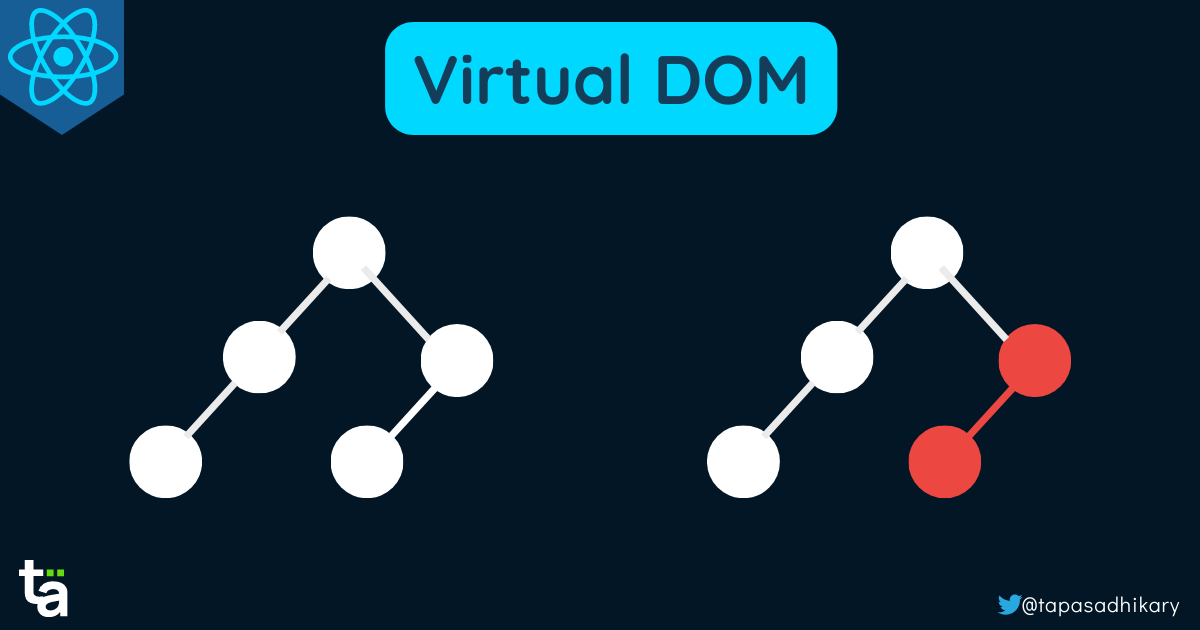
\includegraphics[height=0.3\textheight]{images/virtualDom}}
	\caption{Virtual-DOM}
\end{figure}

Das Bild zeigt schematisch, wie das Virtual DOM in React funktioniert. Zunächst wird eine virtuelle Darstellung des DOMs in Form eines Baumes erstellt. Bei Änderungen an der Benutzeroberfläche wird ein neuer Baum erstellt und mit dem vorherigen Baum verglichen. Dabei werden nur die Unterschiede zwischen den beiden Bäumen ermittelt. Anschließend werden nur die geänderten Elemente im tatsächlichen DOM aktualisiert. Dieser Prozess wird als Reconciliation bezeichnet \cite{ReactVirtualDOM}.

\subsubsection{Komponenten und Props}
React ist eine Bibliothek für die Entwicklung von Benutzeroberflächen, die auf dem Konzept von Komponenten und Props basiert. Eine React-Komponente ist eine eigenständige und wiederverwendbare Einheit einer Benutzeroberfläche, die entweder als Klasse oder als Funktion definiert werden kann. Komponenten können andere Komponenten enthalten und selbst als Teil einer größeren Anwendung verwendet werden \cite{ReactComponentsAndProps}.\\
Props (kurz für "Properties") sind ein wichtiger Mechanismus zur Konfiguration von React-Komponenten. Sie dienen zum Übergeben von Daten von einer Komponente zur anderen und werden als Objekt an die Komponente übergeben. Innerhalb der Komponente können Props als Parameter verwendet werden. Im Gegensatz zum State, der zur Änderung der Benutzeroberfläche innerhalb einer Komponente verwendet wird, sind Props schreibgeschützt und können nicht direkt geändert werden. Durch das Verwenden von Props können Komponenten einfach wiederverwendet werden, indem sie in verschiedenen Kontexten mit unterschiedlichen Props konfiguriert werden \cite{ReactComponentsAndProps}.\\
Ein Beispiel für eine React-Komponente mit Props ist die Funktion \emph{Greeting}, die einen Gruß mit dem Namen des Benutzers anzeigt. Der Name wird als Prop an die Komponente übergeben und innerhalb der Funktion als Parameter verwendet. Hier ist das Codebeispiel:
\begin{lstlisting}[language=vhdl,
	frame=single,           % Ein Rahmen um den Code
	framexleftmargin=15pt,  % Rahmen link von den Zahlen
	style=algoBericht,
	label={Props-Komponenten},
	captionpos=b ,          % Caption unter den Code setzen
	caption={Beispiel Kompoonente mit Probs in React}]
import React from 'react';
	
function Greeting(props) {
   return <h1>Hello, {props.name}!</h1>;
}
	
	export default Greeting;
\end{lstlisting}

Alle React-Komponenten müssen sich im Bezug auf ihre Props als sogenannte "pure functions" verhalten \cite{ReactComponentsAndProps}. Das bedeutet, dass die Funktion der Komponente nur von ihren Props abhängen sollte und keine weiteren Seiteneffekte haben darf. Eine Komponente, die sich wie eine "pure function" verhält, ist leichter zu testen und zu warten.\\
Es gibt auch fortgeschrittene Konzepte im Zusammenhang mit Props, wie das Konzept des "Render Props". Hierbei handelt es sich um eine Technik zum Austauschen von Code zwischen React-Komponenten, bei der eine Komponente eine Funktion als Prop akzeptiert, die ein React-Element zurückgibt. Dadurch können Komponenten dynamisch wiederverwendet werden und die Codebasis der Anwendung wird vereinfacht\cite{ReactRenderProps}.\\
Um mit React-Komponenten und Props zu arbeiten, gibt es verschiedene Möglichkeiten. Funktionskomponenten sind die einfachste Art, eine Komponente zu definieren, indem man eine JavaScript-Funktion schreibt. Klassenkomponenten bieten mehr Funktionen, wie den Zugriff auf den State, die Möglichkeit, Lifecycle-Methoden zu definieren und vieles mehr \cite{RunebookReactComponentsAndProps}.\\
Insgesamt sind Komponenten und Props wichtige Konzepte in React, die Entwicklern helfen, wiederverwendbare Benutzeroberflächenkomponenten zu erstellen und die Effizienz der Entwicklung zu erhöhen.\\
\subsubsection{State}

In React ist der "State" ein Objekt, das in einer Komponente definiert wird und Werte speichert, die zur Laufzeit der Anwendung verändert werden können. Der Zustand wird in der Regel verwendet, um die Darstellung der Benutzeroberfläche zu aktualisieren, wenn sich etwas ändert. Wenn der Zustand eines Komponentenobjekts geändert wird, wird die Methode "render()" aufgerufen, um die Änderungen in der Benutzeroberfläche anzuzeigen \cite{W3SchoolsReactState}.\\

Der Zustand wird oft als Schlüssel-Wert-Paar-Objekt definiert, wobei jeder Schlüssel eine Eigenschaft repräsentiert, die geändert werden kann, und jeder Wert den aktuellen Wert dieser Eigenschaft darstellt. State-Objekte können als eine Art Konfiguration betrachtet werden, die der Komponente zur Verfügung gestellt werden, um ihre Eigenschaften und ihr Verhalten zu steuern \cite{FreeCodeCampStateInReact}.\\
Der Zustand ist ein beobachtbares Objekt und kann somit verändert werden. In React-Komponenten kann der Zustand durch die Verwendung der \emph{setState()}-Funktion aktualisiert werden.\\
Eine sorgfältige Verwaltung des Zustands in einer React-Anwendung ist wichtig, um Fehler zu vermeiden und die Leistung zu optimieren. Die Organisation des Zustands und die Datenfluss zwischen den Komponenten sollten gut durchdacht sein, um überflüssigen oder doppelten Zustand zu vermeiden \cite{ReactManagingState}.\\
Hier ist ein Beispiel, das zeigt, wie der Zustand in React-Komponenten implementiert werden kann:

\begin{lstlisting}[language=vhdl,
	frame=single,           % Ein Rahmen um den Code
	framexleftmargin=15pt,  % Rahmen link von den Zahlen
	style=algoBericht,
	label={State-Fkt.},
	captionpos=b ,          % Caption unter den Code setzen
	caption={Beispiel State in Reeact}]
import React, { useState } from "react";
	
function Example() {
  // Initialisieren des State-Objekts
  const [count, setCount] = useState(0);
  //Erhoehen des Zaehlers, wenn der Button geklickt wird
  function increaseCount() {
    setCount(count + 1);
  }
	
  return (
  <div>
  <p>You clicked {count} times</p>
  <button onClick={increaseCount}>Click me</button>
  </div>
  );
 }
\end{lstlisting}

In diesem Beispiel wird die \emph{useState()} -Hook verwendet, um den Zustand der Komponente zu initialisieren. Die Funktion \emph{useState()} gibt ein Array zurück, das den aktuellen Zustand und eine Funktion zur Aktualisierung des Zustands enthält. In diesem Fall wird der Zustand mit \emph{count} initialisiert und die Funktion \emph{setCount()} wird verwendet, um den Zustand zu aktualisieren. Wenn der Button geklickt wird, wird die \emph{increaseCount()} Funktion aufgerufen, die den Zähler erhöht und den Zustand mithilfe von \emph{setCount()} aktualisiert. Die Änderung des Zustands löst eine erneute Ausführung der Komponente aus, und die aktualisierten Werte werden in der Benutzeroberfläche angezeigt.


\subsection{Verwendung von React}
\subsubsection{Einrichtung von React}
 Eine der einfachsten Möglichkeiten, ein neues React-Projekt zu starten, ist mit einer einfachen HTML-Seite und einigen Skript-Tags \cite{deLegacyReactjs}. Dadurch ist es möglich in kürzester Zeit eine Grundeinstellung erstellen.\\
 Eine andere Möglichkeit, mit der Entwicklung von React-Anwendungen zu beginnen, bietet der \emph{Create-React-App}-Generator\cite{vsCodeReactTutorial}.Der Generator ist eine schnelle und einfache Möglichkeit, neue React-Projekte einzurichten. Um den Generator zu verwenden, wird der folgende Befehl im Terminal ausgeführt:
 
\begin{lstlisting}[language=vhdl,
	frame=single,           % Ein Rahmen um den Code
	framexleftmargin=15pt,  % Rahmen link von den Zahlen
	style=algoBericht,
	label={App-Erstellung},
	captionpos=b ,          % Caption unter den Code setzen
	caption={Beispiel Anwendungserstellung}]
npx create-react-app my-app
cd my-app
npm start
\end{lstlisting}
Durch  Ausführen von \emph{npx create-react-app my-app} wird ein neues React-Projekt mit dem Namen \emph{my-app} erstellt. Mit \emph{cd my-app} wird in das neu erstellte Verzeichnis gewechselt. Anschließend wird die Anwendung mit dem Befehl\emph{npm start} gestartet.
Der Webserver startet und die Anwendung ist unter \emph{http://localhost:3000} im Browser aufrufbar.\\ 
React wurde entwickelt, um keine Annahmen über den Rest des Technologie-Stacks zu treffen. So ist es möglich neue Features zu entwickeln, ohne bestehenden Code umzuschreiben\cite{deLegacyReactjsDocs}. React kann  auf dem Server mit Node oder als mobile Anwendung mit React Native gerendert werden. 
Zusammenfassend lässt sich sagen, dass die Einrichtung von React ein unkomplizierter Prozess ist, mit dem es möglich ist in kurzer Zeit mit der Entwicklung von Benutzeroberflächen für Web- und mobile Anwendungen zu beginnen.

\subsubsection{Komponentenentwicklung}
Die Entwicklung von Komponenten ist ein wichtiger Aspekt bei der Verwendung von React. React-Komponenten sind wiederverwendbare Elemente, die das Erstellen von Benutzeroberflächen erleichtern. Eine React-Komponente implementiert eine \emph{render()}-Methode, die Eingabedaten (Props) nimmt und zurückgibt, was gerendert wird. Es verwendet eine XML-ähnliche Syntax namens JSX, mit der es HTML-ähnlichen Code direkt in JavaScript schreiben kann.\cite{deLegacyReactjs}\\
Ein einfaches Beispiel für eine React-Komponente ist ein "Gruß" (Greeting) Komponente, die eine Begrüßungsnachricht basierend auf dem übergebenen Namen anzeigt:
\begin{lstlisting}[language=vhdl,
	frame=single,           % Ein Rahmen um den Code
	framexleftmargin=15pt,  % Rahmen link von den Zahlen
	style=algoBericht,
	label={Greeting-Komponente},
	captionpos=b ,          % Caption unter den Code setzen
	caption={Beispiel Komponentenentwicklung }]
import React, { Component } from 'react';

class Greeting extends Component {
     render() {
        const { name } = this.props;
        return <h1>Hallo, {name}!</h1>;
    }
}
\end{lstlisting}
In diesem Beispiel wird eine Greeting-Komponente erstellt, die die \emph{render()}-Methode implementiert. Auf die übergebenen Eingabedaten, welche an die Komponente übergeben werden, ist es mittels \emph{this.props} möglich darauf zuzugreifen\cite{deLegacyReactjs}. Mit der JSX-Syntax wird eine Willkommensnachricht direkt in ein HTML-ähnliches Element einfügen. \\

React fördert einen Komponentenentwicklungsansatz, um modulare, wiederverwendbare Benutzeroberflächen zu erstellen. Die Aufteilung der Benutzeroberfläche in kleinere Komponenten erleichtert die Organisation und Wartung des Codes.

\subsubsection{Ereignisbehandlung}
Die Ereignisbehandlung ist ein weiterer wichtiger Aspekt bei der Verwendung von React. Dadurch ist es möglich auf Benutzeraktionen wie Klicks und Tastenanschläge zu reagieren und die Anwendung entsprechend zu aktualisieren.Bei React-Elementen ist die Ereignisbehandlung ähnlich wie bei DOM-Elementen, es gibt jedoch einige syntaktische Unterschiede. Beispielsweise werden die Ereignisse von React in CamelCase statt in Kleinbuchstaben benannt, und JSX übergibt Funktionen als Event-Handler anstelle von Strings.\cite{react_de_handling_events}

Ein einfaches Beispiel für die Ereignisbehandlung in React ist eine Schaltfläche (Button), die bei einem Klick eine Nachricht in der Konsole ausgibt:

\begin{lstlisting}[language=vhdl,
	frame=single,           % Ein Rahmen um den Code
	framexleftmargin=15pt,  % Rahmen link von den Zahlen
	style=algoBericht,
	label={Events},
	captionpos=b ,          % Caption unter den Code setzen
	caption={Beispiel EventHandler}]
import React, { Component } from 'react';

class ButtonClick extends Component {
     handleClick() {
         console.log('Button wurde geklickt!');
     }
 
 render() {
 	return (
 	    <button onClick={this.handleClick}>
 	    Klick mich!
 	    </button>
 	    );
     }
 }

\end{lstlisting}

In diesem Beispiel wird eine \emph{ButtonClick} Komponente erstellt, die die \emph{render()} Methode implementiert und ein \emph{<button>} Element mit einem \emph{onClick Eventhandler} zurückgibt. Der Eventhandler ist die \emph{handleClick} Methode, die in der Komponente definiert ist. Wenn der Benutzer auf den Button klickt, wird die \emph{handleClick} Methode ausgeführt und die Nachricht "Button wurde geklickt!" in der Konsole angezeigt.\cite{react_de_handling_events}\\

Die Ereignisbehandlung in React ermöglicht es, interaktive Benutzeroberflächen zu erstellen und auf Benutzeraktionen dynamisch zu reagieren. Durch die Verwendung von Eventhandlern können Anwendungen auf Benutzerinteraktionen reagieren und den Zustand der Anwendung und die Benutzeroberfläche entsprechend aktualisieren.

\subsubsection{JSX}
JSX ist eine XML-ähnliche Syntax, die von React verwendet wird, um die Benutzeroberfläche einer Anwendung zu definieren \cite{deLegacyReactjs}. JSX ermöglicht es Entwicklern, die Struktur und das Erscheinungsbild von Komponenten ähnlich wie HTML zu beschreiben. Die Verwendung von JSX ist optional,  hat sich jedoch als effizient und bequem für die Arbeit mit React-Komponenten erwiesen.\\
In JSX werden Komponenten als Tags definiert, die HTML-Tags ähneln, mit einigen Unterschieden. Zum Beispiel behandelt React Komponenten in Kleinbuchstaben  als DOM-Tags und Komponenten in Großbuchstaben  als benutzerdefinierte Komponenten\cite{ReactComponentsAndProps}. Dies bedeutet, dass \emph{<div />} ein HTML div-Tag darstellt, während \emph{<Welcome />} eine benutzerdefinierte React-Komponente darstellt, vorausgesetzt, dass \emph{Welcome} im Scope ist.\\
JSX bietet auch die Möglichkeit, JavaScript-Ausdrücke in die Komponentenstruktur einzubetten, indem sie in geschweiften Klammern {} eingeschlossen werden. Diese Ausdrücke können Variablen, Funktionen oder Berechnungen enthalten, die zur Laufzeit ausgewertet werden.\\
Ein weiterer Aspekt von JSX ist das Übergeben von  Daten an Komponenten mithilfe von Eigenschaften. Props können in JSX  wie HTML-Attribute definiert werden und schließen bei JavaScript-Ausdrücken den Wert in geschweiften Klammern ein\cite{deLegacyReactjs}. Innerhalb der Komponente sind diese Props über this.props zugänglich.\\
Beispiel React-Komponente mit JSX: 

\begin{lstlisting}[language=vhdl,
	frame=single,           % Ein Rahmen um den Code
	framexleftmargin=15pt,  % Rahmen link von den Zahlen
	style=algoBericht,
	label={JSX},
	captionpos=b ,          % Caption unter den Code setzen
	caption={Beispiel JSX }]
class Welcome extends React.Component {
        render() {
        	return <h1>Hallo, {this.props.name}!</h1>;
        }
    }

    ReactDOM.render(
    <Welcome name="Max" />,
    document.getElementById('root')
    );
\end{lstlisting}
In diesem Beispiel wird eine benutzerdefinierte React-Komponente namens \emph{Welcome} erstellt, die einen Namen über Props erhält und eine Begrüßungsnachricht mit dem Namen anzeigt.

Insgesamt ist JSX eine leistungsstarke Syntax, die die Arbeit mit React-Komponenten erleichtert und die Entwicklung von Anwendungen effizienter gestaltet. Es ermöglicht Entwicklern, die Struktur ihrer Anwendung auf eine Weise zu definieren, die sowohl intuitiv als auch leicht verständlich ist.	

\subsection{Fortgeschrittene Themen in React}
React bietet eine Vielzahl von fortgeschrittenen Techniken und Bibliotheken, um komplexe Anwendungen zu entwickeln. Einige dieser Techniken sind Redux oder Context API, React Router, React Hooks und serverseitiges Rendern.
\subsubsection{Redux oder Context API}
React Redux und Context API sind zwei beliebte Bibliotheken, die React-basierte Anwendungen für das Datenflussmanagement verwenden können. Beide Bibliotheken dienen dem Zweck, den Zugriff auf Daten zu vereinfachen und den Anwendungsstatus effektiv zu verwalten.\\
Redux ist eine Bibliothek, die den Anwendungszustand in einem zentralen Speicher speichert. Dies vereinfacht den Zugriff auf den Anwendungsweiten Status und macht den Gesamtcode strukturierter. Redux bietet auch die Möglichkeit, den Status zu ändern, indem Aktionen ausgelöst werden, die den Status aktualisieren.\\\cite{scalablepath}
Die folgende Abbildung zeigt das Datenmanagement in Redux:
\begin{figure}[htbp]
	\centering
	\fbox{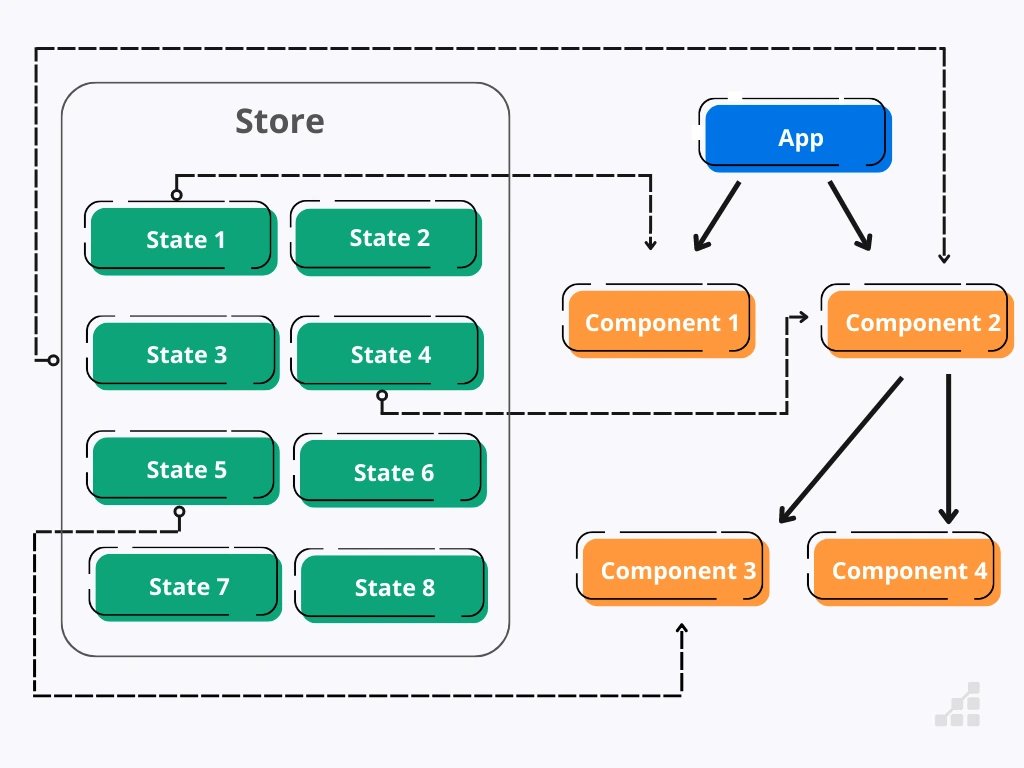
\includegraphics[height=0.3\textheight]{images/redux}}
	\caption{Redux-Datenfluss}
\end{figure}\\
Der Zustand der Anwendung wird im Store gespeichert, der die Datenstruktur und die aktuellen Daten enthält. Die Komponenten erhalten den Zugriff auf den Zustand über das Connect-Modul, das es ihnen ermöglicht, auf die Daten zuzugreifen und sie in ihre Eigenschaften zu übertragen. Wenn ein Ereignis eintritt, das den Zustand ändert, wird eine Action ausgelöst, die eine Reducer-Funktion aufruft, um den Zustand im Store zu aktualisieren.\\

Redux eignet sich besonders für Anwendungen mit vielen Komponenten und komplexen Datenstrukturen. Der Hauptvorteil von Redux besteht darin, dass das Datenflussmanagement einheitlich und leicht verständlich ist. Dies vereinfacht die Anwendungswartung erheblich, da Entwickler immer genau wissen, wo ihr Anwendungsstatus gespeichert ist und wie sie darauf zugreifen können.\\

Die Kontext-API ist eine Redux-Alternative, mit der Entwickler  den Status in ihrer Komponentenhierarchie verwalten können. Die Kontext-API erleichtert den Zugriff auf den Status, indem sie ermöglicht, dass er in der gesamten Komponentenhierarchie weitergegeben wird. Im Gegensatz zu Redux ist die Context-API jedoch nicht gut für Anwendungen mit komplexen Datenstrukturen und  vielen Komponenten geeignet.\\\cite{scalablepath}
Die folgende Abbildung zeigt den Datenfluss in Context API:\\
\begin{figure}[htbp]
	\centering
	\fbox{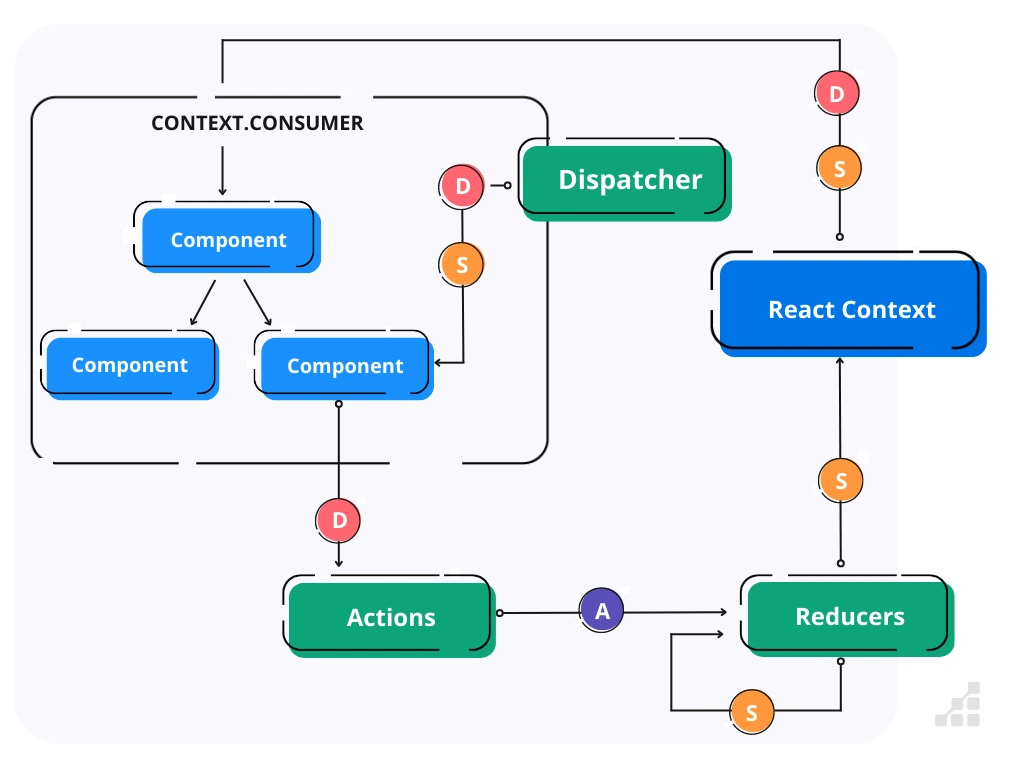
\includegraphics[height=0.3\textheight]{images/context-api}}
	\caption{ContextApi-Datenfluss}
\end{figure}\\
Der Zustand wird in einer höheren Komponente gespeichert und durch die Prop-Drilling-Technik an untergeordnete Komponenten übermittelt. Dadurch können untergeordnete Komponenten den Zustand der höheren Komponenten ändern und somit auch den Zustand der Anwendung beeinflussen.\\
Die Kontext-API eignet sich am besten für Anwendungen, bei denen der Zustand nicht zu komplex und die Anzahl der Komponenten begrenzt ist. Der Hauptvorteil der Kontext-API besteht darin, dass sie eine einfachere und schnellere Möglichkeit bietet, auf den Status zuzugreifen, ohne einen globalen Speicher einrichten und verwalten zu müssen.\\\cite{scalablepath}
Insgesamt eignet sich Redux  für große Anwendungen mit vielen Komponenten und  komplexen Datenstrukturen, während die Context-API für kleine Anwendungen mit einer begrenzten Anzahl von Komponenten und einem einfachen Datenmodell geeignet ist. Beide Bibliotheken sind jedoch nützliche Tools für ein effektives Datenflussmanagement in React-basierten Anwendungen.\cite{scalablepath}
\subsubsection{React Router}
React Router ist eine JavaScript-Bibliothek, die in Verbindung mit der React-Bibliothek verwendet wird.Es ermöglicht   eine effiziente und reibungslose Navigation zwischen verschiedenen Seiten oder Komponenten innerhalb einer Webanwendung.\\ 
Die Verwendung von React Router bringt viele Vorteile für das Design und die  Entwicklung von Webanwendungen.\\
Erstens können Inhalte dynamisch angezeigt werden, ohne  die gesamte Seite neu zu laden. Dies sorgt für eine schnellere und einfachere Erfahrung für  Endbenutzer. Zweitens trägt es dazu bei, das Layout der Anwendung sauber und gut strukturiert zu halten, indem es die Navigation zwischen den verschiedenen Komponenten einer Anwendung erleichtert.\\
React Router verwendet eine hierarchische Struktur, um die Navigation innerhalb der Anwendung zu organisieren.Dazu können  mehrere Unterthemen bzw. Komponenten zu einem Oberthema bzw. Hauptkomponente zusammengefasst und  für jedes dieser Unterthemen unterschiedliche Routen definiert werden.\\
Auf diese Weise können Entwickler ihre Anwendungen modularisieren und gleichzeitig ihre Wartbarkeit und Skalierbarkeit  sicherstellen.\\
Um React Router in einer React-Anwendung zu verwenden, muss  zuerst die React-Router-Dom-Bibliothek installiert werden. Dies kann durch Ausführen des Befehls \emph{npm i -D respond-router-dom} in einem Terminal  im Stammverzeichnis der Anwendung erreicht werden.Anschließend ist es möglich mit React Router verschiedene Routen und Komponenten zu definieren und zu verknüpfen, um eine effiziente und benutzerfreundliche Navigation innerhalb einer Anwendung zu gewährleisten.\\
Zusammenfassend ist React Router eine praktische und weit verbreitete Bibliothek, mit der es möglich ist eine effiziente Navigation und Routenverwaltung in einer React-Anwendungen implementieren zu können. So eine einfach zu integrierende und modulare Struktur ermöglicht es Entwicklern, schnell und einfach attraktive und einfach zu bedienende Webanwendungen zu erstellen.\cite{react-router}

\subsubsection{React Hooks}
React Hooks ist eine revolutionäre Funktion, die in React Version 16.8.0 eingeführt wurde.Es ist  Entwicklern möglich, Status- und andere React-Funktionen in funktionalen Komponenten zu verwenden, ohne Klassenkomponenten schreiben zu müssen.\\
React Hooks haben gegenüber Klassenkomponenten mehrere Vorteile. Zu mal ist die Syntax einfacher und leichter  zu verstehen, wodurch Ihr Code leichter zu lesen und zu warten ist. Zu dem erleichtert es die gemeinsame Nutzung von Logik zwischen Komponenten, ohne dass komplexe Entwurfsmuster wie Komponenten höherer Ordnung und Render-Props erforderlich sind.\\
Die in React verfügbaren grundlegenden Hooks sind die Hooks \emph{useState} und \emph{useEffect}. Mit dem \emph{useState}-Hook können Sie den lokalen Status funktionaler Komponenten verwalten und  aktualisieren. Der \emph{useEffect}-Hook hingegen wird  in funktionalen Komponenten verwendet, um Seiteneffekte wie Datenabruf und Ereignisabonnements zu behandeln.\\  
Um Hooks in einer React-Anwendung zu verwenden, müssen   die entsprechenden Hooks zuerst aus der React-Bibliothek importiert werden. Diese Hooks können dann innerhalb funktionaler Komponenten verwendet werden, um den gewünschten Zustand oder Nebeneffekte zu verwalten. Es ist wichtig zu beachten, dass Hooks nur innerhalb von Funktionskomponenten verwendet werden können, nicht innerhalb von Klassenkomponenten oder JavaScript-Funktionen. \cite{react-hooks}\\
Zusammenfassend sind React Hooks eine leistungsstarke und innovative Funktion, die es Entwicklern ermöglicht, den Status von Funktionskomponenten und anderen React-Funktionen effizient zu verwalten.  React Hooks verändern und vereinfachen grundlegend die Art und Weise, wie React-Anwendungen entwickelt werden, indem sie eine einfache Integration und verbesserte Code-Lesbarkeit bieten.

\subsubsection{Serverseitiges Rendern}
Serverseitiges Rendering (SSR) ist ein wichtiger Aspekt der React-Anwendungsentwicklung, der es ermöglicht, React-Komponenten auf dem Server zu rendern, bevor das vollständig gerenderte HTML-Dokument an den Client gesendet wird [2].
Die Herausforderung beim Erstellen von Webanwendungen besteht darin, ein optimales Benutzererlebnis zu gewährleisten und gleichzeitig die Sichtbarkeit in Suchmaschinen zu erhöhen. Serverseitiges Rendering bietet hierfür eine Lösung.\\

\begin{figure}[htbp]
	\centering
	\fbox{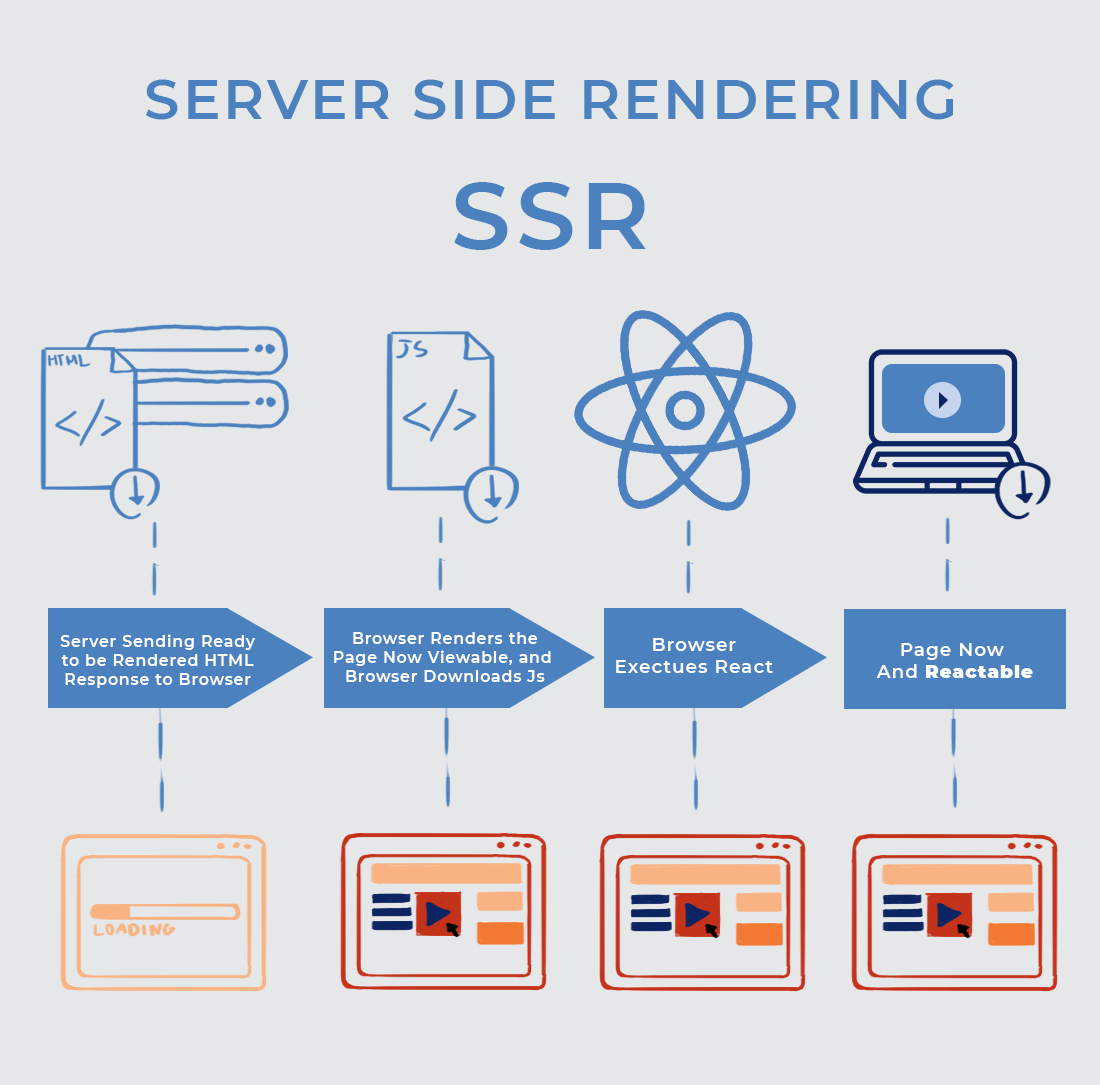
\includegraphics[height=0.3\textheight]{images/ssr}}
	\caption{SSR in React}
\end{figure}
Der Prozess des serverseitigen Renderns in React kann in vier Schritten zusammengefasst werden, wie im angegebenen Bild dargestellt:\\
\begin{itemize}
	\item[1.] {Der Client sendet eine HTTP-Anfrage an den Server}
	\item[2.]  {Der Server rendert die React-Komponenten der Seite in einen HTML-String.}
	\item[3.]  {Der Server injiziert den gerenderten HTML-String in ein HTML-Dokument.}
	\item[4.]  {Der Server sendet das vollständig gerenderte HTML-Dokument an den Client.}
\end{itemize}
Um serverseitiges Rendering in einer React-Anwendung zu implementieren, muss ein eigener Backend-Server entwickeln werden. Die Serverintegration von Node.js ist in diesem Zusammenhang eine gängige Lösung. Darüber hinaus sind möglicherweise weitere Anpassungen erforderlich, z. B. die Verwendung von serverseitigem Rendering mit React Router.\cite{Drehmanns2021}\\

Zusammenfassend lässt sich sagen, dass serverseitiges Rendering eine nützliche Technik zur Verbesserung der Leistung und Suchmaschinenoptimierung von React-Anwendungen ist. Indem Sie Ihre Anwendung auf dem Server rendern und das vollständig gerenderte HTML-Dokument an den Client senden, können Sie die anfänglichen Ladezeiten verkürzen und die Sichtbarkeit Ihrer Anwendung in Suchmaschinen erhöhen.

\subsection{Best Practices in React-Entwicklung}
 Bei der Entwicklung von React-Anwendungen ist es entscheidend, bewährte Methoden und Best Practices einzuhalten, um skalierbare, wartbare und effiziente Anwendungen zu erstellen. Einige dieser Best Practices beziehen sich auf das Verwenden von Werkzeugen und Bibliotheken, die die Produktivität steigern und die Codequalität verbessern. 
\subsubsection{Testen von React-Anwendungen}
Das Testen von React-Anwendungen ist ein wichtiger Aspekt, um die Codequalität und Zuverlässigkeit in der Softwareentwicklung sicherzustellen. Es gibt verschiedene Testmethoden und Tools, die auf verschiedene Aspekte einer Anwendung abzielen.\\
\begin{figure}[htbp]
	\centering
	\fbox{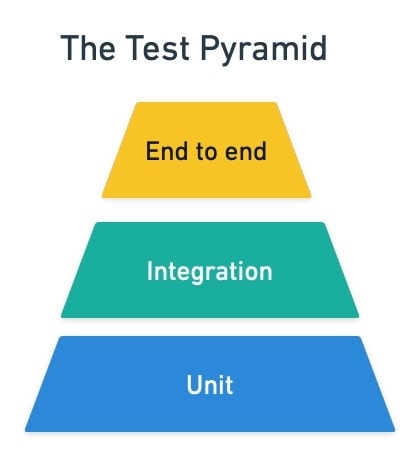
\includegraphics[height=0.3\textheight]{images/pyramid}}
	\caption{SSR in React}
\end{figure}
Die oben abgebildete Testpyramide ist ein Konzept, welches zur Erstellung verschiedener Testmethoden hilft.Dazu gehören End-to-End-Tests (E2E), Integrationstests und Komponententests (Unit-Tests). Unit-Tests werden für kleine, isolierte Codeblöcke wie einzelne Funktionen oder Komponenten verwendet und konzentrieren sich auf das Testen von Teilaspekten der Anwendung.\\
Ein beliebtes Tool zum Testen von React-Anwendungen ist die React Testing Library (RTL). RTL konzentriert sich darauf, die Komponente aus der Sicht des Endbenutzers zu testen, anstatt die Implementierung und Logik der zugrunde liegenden React-Komponente zu validieren. Auf diese Weise können Entwickler sicherstellen, dass ihre Anwendungen für ihre Benutzer wie erwartet funktionieren.\cite{react-test-runebook}\\ 
Jest ist ein weiteres beliebtes Testtool, das speziell zum Testen von React-Anwendungen entwickelt wurde.Jest ordnet und strukturiert die Testsuite und überprüft die gewünschten Eigenschaften. In Kombination mit Enzyme, das den zu testenden Frontend-Code ausführt und die relevanten Schnittstellen bereitstellt, ermöglicht Jest Entwicklern den Zugriff auf und die Interaktion mit den generierten Elementen.\cite{react-test-ix}\\

Zusammenfassend lässt sich sagen, dass das Testen von React-Anwendungen ein wichtiger Teil des Entwicklungsprozesses ist, der dazu beiträgt, die Codequalität sicherzustellen und potenzielle Fehler frühzeitig zu erkennen. Durch die Verwendung von Testwerkzeugen wie der React Testing Library und Jest in Verbindung mit den Prinzipien der Testpyramide können Entwickler umfassende Tests durchführen, um sicherzustellen, dass sich ihre Anwendungen wie erwartet verhalten.

\subsubsection{Performance-Optimierung}
Die Performance-Optimierung ist ein Schlüsselfaktor bei der Entwicklung von React-Anwendungen, um eine schnelle und reaktionsschnelle Benutzererfahrung zu erreichen. Es gibt verschiedene Ansätze und Techniken, um die Leistung von React-Anwendungen zu optimieren.\\
Eine gängige Methode zur Verbesserung der Leistung in React ist die Verwendung von \emph{React.PureComponent}. Anstatt ein eigenes \emph{shouldComponentUpdate} zu schreiben, ist es möglich \emph{React.PureComponent} zu verwenden, um unnötiges Rendern von Komponenten zu verhindern. \emph{React.PureComponent} führt einen flachen Vergleich von Props und State durch. In vielen Fällen reicht dies aus, um unnötige Updates zu vermeiden.
Es ist jedoch wichtig zu beachten, dass React.PureComponent möglicherweise nicht geeignet ist, wenn Props oder State auf eine Weise mutiert werden, die bei einem oberflächlichen Vergleich übersehen würde.\\
Neben der Verwendung von \emph{React.PureComponent} ist es wichtig, die Gesamtleistung der Webanwendung zu berücksichtigen. Beispielsweise kann die Optimierung von CSS-Dateien einen erheblichen Einfluss auf die Anwendungsleistung haben. In einem Testfall benötigte der Browser über 50 ms, um die zweite doppelt eingebettete CSS-Datei von 25 KiB zu interpretieren und die Regeln korrekt anzuwenden, während die erste Datei nur 6 ms brauchte. Dies unterstreicht, wie wichtig es ist, Ressourcen sorgfältig zu verwalten und unnötige Doppelarbeit zu vermeiden.\cite{react-performance}\\

Insgesamt ist die Optimierung der Leistung Ihrer React-Anwendung ein wichtiger Aspekt, um eine schnelle und reaktionsschnelle Benutzererfahrung sicherzustellen. Die Verwendung von Techniken wie \emph{React.PureComponent} und die Optimierung von Ressourcen wie CSS-Dateien können die Anwendungsleistung verbessern und die beste Benutzererfahrung gewährleisten.\cite{css-performance}\\


\subsubsection{Sicherheit und React}
Wenn es um Sicherheit geht, bietet React einige integrierte Funktionen, um häufige Web-Sicherheitsprobleme zu vermeiden. Allerdings liegt es  auch in der Verantwortung des Entwicklers, für die Sicherheit der Anwendung zu sorgen.\\

React rät beispielsweise von der Verwendung unsicheren Codes ab, indem es JSX bereitstellt, das  Ausdrücke vor dem Rendern standardmäßig maskiert, um Cross-Site-Scripting-Angriffe (XSS)  zu verhindern. Es soll jedoch beachtet werden, dass ReactJS selbst keine vollständige Sicherheitslösung ist. Auch auf andere Sicherheitsaspekte wie sichere API-Endpunkte und den richtigen Einsatz von HTTPS sollten Entwickler bewusst achten.\\

Darüber hinaus gibt es Tools wie „Invicti Web Application Security Scanner“, die  automatische Schwachstellenprüfungen durchführen und dabei helfen, die Sicherheit von React-Anwendungen weiter zu verbessern\cite{geekflare_learning_resources}\cite{geekflare_rendering}.\\

Insgesamt bietet React  eine solide Grundlage für die sichere Entwicklung von Webanwendungen,  erfordert jedoch von den Entwicklern dennoch ein hohes Maß an Bewusstsein und Sorgfalt, um sicherzustellen, dass ihre Anwendungen resistent gegen Angriffe sind.\\

\subsection{Vergleich mit anderen Frontend-Technologien}
In diesemm Kapitel werden die unterschiedlichsten Frontend- Technologien miteinander verglichen.
\subsubsection{Vor- und Nachteile von React im Vergleich zu Angular und Vue.js}
React, Angular und Vue.js sind beliebte Frontend-Technologien, die bei der Entwicklung von modernen Webanwendungen eingesetzt werden. Jede Technologie hat ihre Vor- und Nachteile, die bei der Wahl der Technologie berücksichtigt werden sollten.
Angular, React und Vue.js sind alle weit verbreitet und haben jeweils ihre Stärken und Schwächen.\\

Angular ist ein umfangreiches Framework zum Erstellen skalierbarer und leistungsstarker Anwendungen. Es verfügt über einen schlanken Kerncode mit hoher Modularität mit externen Komponenten, was eine unbegrenzte Integration und Nutzung von HTML und CSS ermöglicht. Darüber hinaus unterstützt es TypeScript und JavaScript und trennt Vorlagen strikt  von Design und Logik \cite{hosttest2021}. Der Nachteil ist, dass frühere Angular-Versionen nicht gut für den Aufbau dynamischer Webanwendungen und  komplexer digitaler Produkte  geeignet sind \cite{ichi2023}.\\

React hingegen ist eine Open-Source-GUI-Bibliothek und bietet einige Vorteile. Neue Entwickler können dieses Tool leicht erlernen. Es kann mit anderen JS-Bibliotheken und Frameworks verwendet werden \cite{softwaredeveloperindia2022}. React verfügt außerdem über eine sehr aktive Community, die ständig neue Bibliotheken und Tools entwickelt, um die Entwicklung einfacher und schneller zu machen. Der Nachteil ist, dass es  nicht so leistungsstark ist wie Angular oder Vue \cite{logrocket2021}.

Vue.js ist dasjenige neueste der drei Frameworks und zeichnet sich durch eine einfache Satzlehre und eine leichte Lernkurve aus. Es hat eine sehr schnelle Startzeit und ist daher unter Entwicklern beliebt, selbige schnell Prototypen hinstellen möchten\cite{logrocket2021}. Obwohl Vue.js eine kleinere Community hat denn Angular und React, wächst jene schnell und bietet eine starke Unterstützung \cite{codeinwp}.

Diese Vor und Nachteile werden in der nachfolgenden Tabelle nochmals visualisiert.
\begin{center}
\begin{table}[h]
	\begin{tabularx}{4cm}{|l|l|p{4.5 cm}|ll}
		\cline{1-3}
		\textbf{Technolgie} & \textbf{Vorteil}                         & \textbf{Nachteil}                                                &  &  \\ \cline{1-3}
		Angular             & Schlanker Kerncode mit hoher Modularität & nicht geeignet für dynamiche Web-App  &  &  \\ \cline{1-3}
		React               & Einfach zu erlernen, aktive Community    & Weniger leistungsstark         &  &  \\ \cline{1-3}
		Vue.js              & Einfache Satzlehre, schnelle Startzeit   & Kleinere Community             &  &  \\ \cline{1-3}
	\end{tabularx}
\end{table}
\end{center}

Zusammenfassend haben alle drei Frameworks ihre eigenen Stärken und Schwächen haben und die Wahl hängt deutlich von den spezifischen Erwartungen und Präferenzen des Entwicklerteams ab.

\subsection{Fazit}
React hat sich als eine der beliebtesten JavaScript-Bibliotheken etabliert und bietet Entwicklern eine effiziente und flexible Plattform zum Erstellen von Benutzeroberflächen für Webanwendungen. Es zeichnet sich durch die Bereitstellung wiederverwendbarer UI-Komponenten und einer deklarativen Codestruktur aus, die das Debuggen und die Vorhersagbarkeit erleichtert. 
Die Weiterentwicklung von React zeigt deutlich, dass der Trend zur Verwendung von React Hooks weiter zunimmt. Sie bieten eine einfachere und effizientere Möglichkeit zur Erstellung von React-Komponenten  und werden bereits von vielen Unternehmen in der Produktion eingesetzt. Es wird erwartet, dass dieser Trend die Zukunft der React-Entwicklung  prägen wird.  React lebt in einem dynamischen Ökosystem und interagiert mit anderen Technologien und Frameworks. Neuere Technologien wie Svelte verfolgen einen anderen Ansatz bei der Nutzung des virtuellen DOM und könnten zu zukünftigen Verbesserungen und Änderungen an React führen. 
Zusammenfassend lässt sich sagen, dass React aufgrund seiner Flexibilität, Beliebtheit und aktiven Community  eine starke Position in der Zukunft der Webentwicklung einnehmen könnte. Es wird erwartet, dass React seine Rolle als Branchenführer beibehält und weiterhin innovative Lösungen für die Entwicklung von Benutzeroberflächen bereitstellt.

\section{Docker}

\begin{wrapfigure}{r}{0.4\textwidth}
\centering
\fbox{
\includegraphics[width=0.30\textwidth]{images/docker}}
\end{wrapfigure}

Um die DHBW Star Webseite Plattformunabhängig testen und betreiben können, entschieden wir uns für Docker. Dieser ist sowohl auf unseren Rechnern als auch auf dem Test Server installiert. Damit wurden Probleme, die durch unterschiedlichen Betriebssysteme oder Softwareversionen entstehen könnten, vermieden.

\subsection{Docker Grundlagen}

Docker ist eine freie Container basierte Virtualisierung Software unter der Apache-Lizenz.
Docker kann eine Software mit all ihren benötigten Abhängigkeiten (z.B. Bibliotheken) in ein Containerimage packten. Dieses Image kann Docker unabhängig von der Plattform oder der vorhandenen Software ausführen. Dies Ermöglicht einen hohen Grad an Flexibilität, erhöht die Sicherheit und verhindert Probleme mit verschieden Versionen von Bibliotheken.
Jeder Container ist eine eigene Sandbox und Somit Isoliert und unabhängig von anderen Prozessen auf dem Host System.

\subsection{Docker Images und Container}
Um ein Programm in Docker zu starten werden zwei Schritte benötigt.\\
1. Ein Docker Images erzeugen.\\
2. Image als Container Starten.\\
Um ein Image zu erstellen wird meist ein Vorhandenes als Basis-Image verwendet. Dockerhub.com biete eine Vielzahl an Images für alle möglichen Anwendungen an.
In einer Datei mit den Namen Dockerfile kann mit \emph{FROM "imagename"} eins der Images einfach als Basis festgelegt werden. Danach können eigene Dateien kopiert oder Programme installiert bzw. Ausgeführt werden. Diese Änderungen gespeichert einen Virtuellem Dateisystem im erzeugtem Image.

Wenn ein Image gestartet wird nennt Docker dies einen Container.
Beim Starten können noch Einstellungen festgelegt werden (z.B. Port Weiterleitung).
Jedes Image kann beliebig oft als Container mit eigenen Einstellungen gestartet werden. So ist es möglich, das selbe Image mit unterschiedlicher Konfiguration gleichzeitig laufen zu lassen.

\todo {Quelle: docs.docker.com}

\subsection{Docker Compose}
Gehören zu einer Anwendung oder einem Service mehrere Container so bietet der Client \emph{Docker Compose} die Möglichkeiten automatisch Images zu erzeugen und Container zu starten. Dafür wird in der \emph{compose.yaml} Datei die zu startenden Container und die jeweils dazugehörige Konfiguration angeben.
Mit dem Befehl \emph{docker compose up} starten alle Container.
Dadurch wird ein hoch automatisierter Arbeitsprozess ermöglicht.

\subsection{Vor- und Nachteile von Docker}
Docker ermöglicht durch seine flexible Abstraktion ein fast plattformunabhängigen betrieb von Software. Dies wird erreicht in dem Docker verschiedenen Ebenen von Abstraktionen verwendet um so für die Software eine einheitliche Umgebung zu garantieren. Es wir aber im Gegensatz zu Virtuellen Maschinen keine Hardware simuliert.


Für Abstraktion werden allerdings mehr Ressourcen benötigt, da teilweise ganze Betriebssysteme in einem Container laufen. Somit kann ein einzelner Docker Container gern mal mehrere GB an Arbeitsspeicher benötigen.

Zudem kann das bauen eines Containers je nach Rechenleistung einiges an zeit in Anspruch nehmen. Das kann vor allem beim entwickeln viel zeit kosten, wenn zum testen der Container mehrmals in kurzer Zeit neu gebaut werden muss.

\subsection{Docker unter Windows}
Um Docker unter Windows benutzen zu können muss WSL2 (Windows Subsystem for Linux 2) Installiert und Aktiviert sein.
In diesem läuft dann der Docker Dienst.

Docker Desktop ist eine Client mit Grafische Oberfläche. Dieser steuert den Docker-Dienst um Container zu starten oder zu Stoppen.

Nach dem Start zeigt er die Container welche Docker gespeichert hat mit Namen, Images, Ports und wann er zuletzt gestartet wurde. (Abb: \ref{fig-docker-desktop})
Mit einem Klick auf den Container können unter anderem seine Logs oder ein Terminal im Container erreicht werden, welche bei der Fehlersuche ein sehr hilfreich sein können.

\begin{figure}[htbp]
	\centering
	\fbox{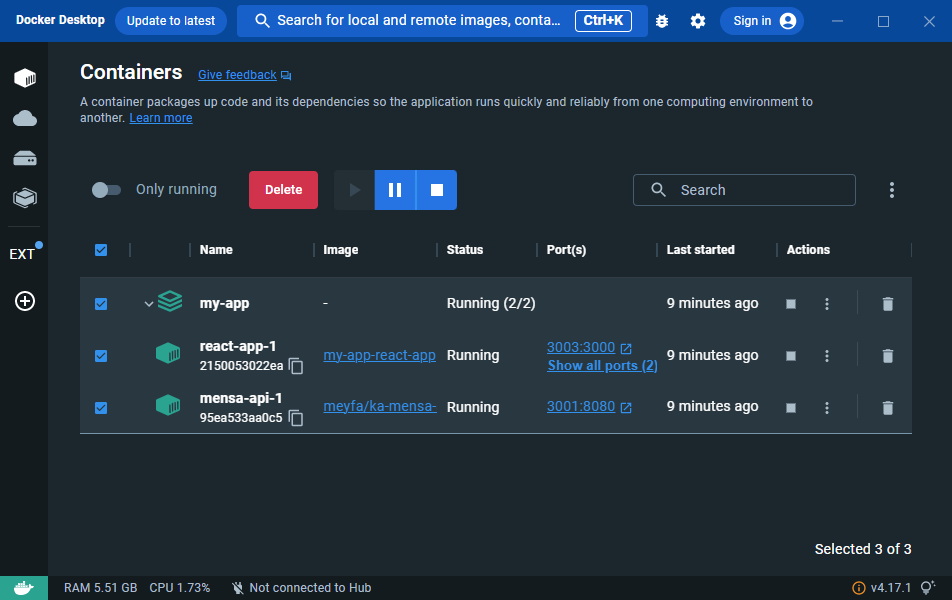
\includegraphics[width=0.9\textwidth]{images/docker-desktop}}
	\caption{\label{fig-docker-desktop} Docker Desktop Screenshot}
\end{figure}

%%%%%%%%%%%%%%%%%%%%%%%%%%%%%%%%%%%%%%%%%%%%%%%%%%%%%%%%%%%%%%%%%%%%%%%%%%%%%%%

\chapter{Umsetzung der Webseite}
Die Digitalisierung hat enorme Auswirkungen auf Bildung und Lehre, und Hochschulen bilden da keine Ausnahme. Die DHBW Karlsruhe setzt sich, wie viele andere Bildungseinrichtungen auch, für die Nutzung digitaler Technologien ein, um das Lernen und die Bewältigung des Hochschullebens zu erleichtern. In diesem Zusammenhang entstand die Idee einer modernen Webseite, die speziell auf die Bedürfnisse der Studierenden der DHBW Karlsruhe zugeschnitten ist. Diese moderne Webseite soll die wichtigsten Informationen, die Studierende benötigen, auf effiziente und benutzerfreundliche Weise zusammenfassen.\\
\section{Ziel der Webseite}
Das Hauptziel der App besteht darin, den Informationsfluss zu optimieren und den Zugriff auf relevante Daten zu erleichtern. Ob Mensa-Speiseplan, aktuelle Vorlesung, Wochenplan oder eine Ansammlung von Links. Die Webseite sollte all diese Informationen an einem  zentralen Ort bereitstellen. Darüber hinaus möchten wir eine intuitive und ansprechende Benutzererfahrung bieten, die den Benutzern den Zugriff und die Navigation erleichtert.\\
\newpage
\subsection{Wissenschaftliche Erkenntnisse} 
Zu den drei Hauptinformationen, die den Nutzern der DHBW Karlsruhe am wichtigsten sind, gehören Speisepläne, Stundenpläne und eine Sammlung nützlicher Links.\\
Der Kantinenplanung kommt eine große Bedeutung zu, da sie es Studierenden der DHBW Karlsruhe ermöglicht über den Tagesplan Bescheid zu wissen.\\
Auch Stundenpläne spielen eine wichtige Rolle, da sie den Studierenden helfen, ihre Kurse und Vorlesungen zu überschauen  und einen Überblick über ihre wöchentlichen Aktivitäten zu erhalten.\\ 
Darüber hinaus ist die Sammlung nützlicher Links eine wertvolle Ressource. Über diese Links erhalten Studierende einen einfachen Zugriff auf wichtige Online-Ressourcen und -Dienste, die sie regelmäßig nutzen. Dies ermöglicht einen schnellen Zugriff auf Informationen und unterstützende Materialien im Zusammenhang mit Ihren Lernbedürfnissen.\\ 
Insgesamt sind Mensapläne, Stundenpläne und eine Sammlung weiterführender Links die drei Hauptinformationen, die wir auf Basis unserer Erfahrung  für Studierende der DHBW Karlsruhe als am wichtigsten erachten. Durch die Optimierung dieser Informationen können Benutzer ihre täglichen Mahlzeiten einsehen, Unterrichtspläne effektiv überblicken und auf wichtige Online-Ressourcen zugreifen, um ihre Lernanforderungen zu erfüllen.\\
Die effektivsten Informationsquellen sind diejenigen, die den Benutzern einen schnellen und einfachen Zugriff auf die benötigten Informationen ermöglichen. In diesem Zusammenhang sind moderne  Webseiten , die auch für mobile Geräte optimiert ist, eine ideale Lösung, da sie die Möglichkeit bieten, alle notwendigen Informationen an einem Ort zu sammeln und sie den Benutzern jederzeit und überall zur Verfügung zu stellen.\\
Das Hauptproblem des Informationsangebots der DHBW Karlsruhe besteht in der Fragmentierung  und dem erschwerten Zugriff auf spezifische Informationen, da diese auf verschiedenen Plattformen verbreitet sind. Unser Vorschlag zur Lösung dieser Probleme ist die Entwicklung mobiler Webseiten. Diese Anwendung verbessert das Benutzererlebnis, indem sie die benötigten Informationen zentralisiert und es Benutzern ermöglicht, die benötigten Informationen schnell und einfach zu finden und zu verwenden.\\ 

\newpage
\section{Grundkonzept der Webseite}
Als mobile Informationsplattform konzipiert, zielt die Webseite darauf ab, die Informationsbeschaffung für Studierende der DHBW Karlsruhe zu optimieren und zu zentralisieren. Durch die Bündelung einer Vielzahl zusammengehöriger Dienste und Informationen und deren Darstellung auf einer intuitiven Benutzeroberfläche wollen wir den Informationsfluss optimieren und gleichzeitig einen hohen Komfort gewährleisten.
\subsection{Benutzeroberfläche}
Das Design der Benutzeroberfläche folgt den Designprinzipien Usability und User Experience (UX)  mit dem Ziel,  intuitive und benutzerfreundliche Anwendungen zu entwickeln\cite{hartmann2017usability}. Diese Prinzipien sind  für die Erstellung effizienter und effektiver Anwendungen, die die Benutzerzufriedenheit erhöhen, von wesentlicher Bedeutung\cite{14all}. Es orientiert sich an zeitgenössischen Designstandards und ist klar und minimalistisch gestaltet,da es dazu beiträgt, dass die Benutzeroberfläche übersichtlich und selbsterklärend bleibt\cite{massiveart}
Die wichtigsten Informationen und Dienste wie Speisepläne, Fahrpläne und Links sind direkt über die Startseite der Webseite zugänglich und werden mit sofort erkennbarer Ikonographie angezeigt..Dies erleichtert Benutzern die Navigation auf Ihrer Website und das Auffinden der benötigten Informationen. Durch die  Verwendung von Ikonografie zur Darstellung dieser Dienste sind diese sofort erkennbar und lassen sich in die Anwendung einfacher verwenden\cite{99designs}. 



\subsection{Navigation und Struktur}
Die Anwendung verwendet ein Seitenmenü zur Navigation. Dieses Menü enthält Symbole, die die Hauptbereiche der Anwendung darstellen, wie z. B. den Speiseplan, den Stundenplan und verschiedene Links.Durch Auswahl eines dieser Symbole gelangt der Benutzer direkt zu den entsprechenden Informationen. Diese Navigationsverwendung sorgt für eine uneingeschränkte  Anzahl von Menüpunkten, die sortierung der Menüpunkte nach Wichtigkeit un der Inhalt der Webseite beginnt direkt am oberen Rand und hat keine Einschränkung\cite{eology2023}.
Darüber hinaus ist die Struktur der Webseite logisch und hierarchisch aufgebaut, mit Seiten, die weitere Details oder spezifische Informationen bieten. Benutzer können zwischen diesen Seiten navigieren, indem sie wischen oder die entsprechenden Optionen in den Menüs auswählen.

\subsection{Funktion und Komponenten}
Die Webseite enthält verschiedene Funktionen und Komponenten, die darauf abzielen, Informationen effektiv anzuzeigen und gleichzeitig ein hohes Maß an Benutzerfreundlichkeit zu gewährleisten. 

Zu den Hauptmerkmalen gehören: 
\begin{itemize}
	\item Speiseplan: Diese Funktion zeigt das Tagesmenü an. Benutzer können sich auch zukünftige Menüs anzeigen lassen.
	\item Stundenplan: Eine Funktion, die den Stundenplan anzeigen lässt.
	\item Links: Diese Funktion bietet eine Sammlung verwandter Links, die Benutzern den einfachen Zugriff auf wichtige Online-Ressourcen und -Dienste ermöglichen.
\end{itemize}
\newpage
\section{Website-Komponenten}
In diesem Kapitel werden die einzelnen Funktionen und Komponenten erläutert-
\subsection{Home}
\subsubsection{Konzept}
Die Homepage ist als zentrale Informations- und Navigationsplattform konzipiert.Diese bietet einen  Überblick über die wichtigsten Informationen und Funktionen und dient gleichzeitig als Ausgangspunkt für die Navigation zu spezifischeren Seiten und Funktionen.  
Die Homepage ist in drei Hauptbereiche unterteilt.
\begin{itemize}
	\item Header:Die Kopfzeile enthält das Logo der Webseite sowie ein die Copyright Bezeichnung auf der rechten Seite. 
	\item Navigation: Die Navigation ist  in vertikaler Form am rechten Rand der Webseite konzipiert. Die enthält die Menüitems mit Symbolen, die den Hauptfunktionen der Webseite entsprechen. Durch Klicken auf diese Symbole gelangt der Benutzer direkt zur entsprechenden Seite.
	\item  Hauptbereich: Im Hauptbereich werden die Informationen angezeigt, die aktuell am relevantesten sind. Dazu gehören <die Angabe der jetzigen Vorlesung, der Mensaplan für den aktuellen Tag und eine Information für die aktuele Zeit.
\end{itemize} 
In dieser Abbildung ist die Visualisierung der Homepage dargestellt.\newpage
\begin{figure}[htbp]
	\centering
	\fbox{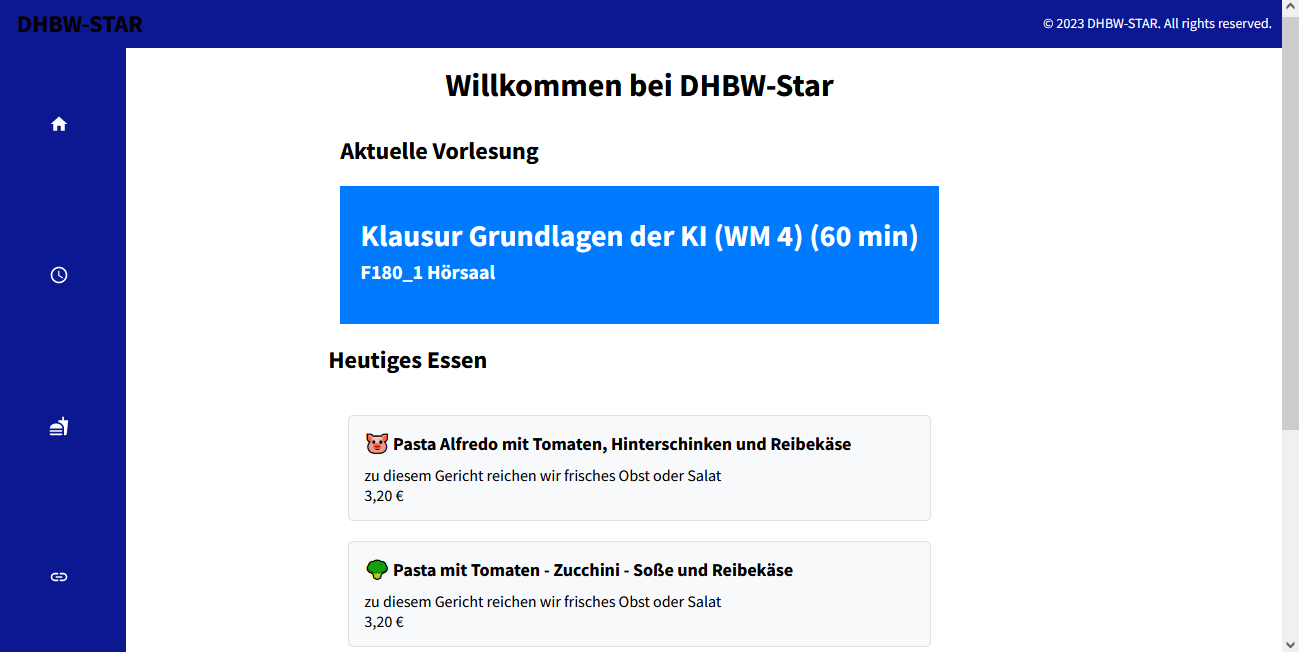
\includegraphics[height=0.3\textheight]{images/homepage}}
	\caption{Homepage}
\end{figure}
\subsubsection{Implementierung}
In diesem Codeblock befindet sich die Homepage-Komponente:\\
\begin{lstlisting}[language=JavaScript,
	frame=single,           % Ein Rahmen um den Code
	framexleftmargin=15pt,  % Rahmen link von den Zahlen
	style=algoBericht,
	label={Homepage-Komponente},
	captionpos=b ,          % Caption unter den Code setzen
	caption={Homepage-Komponente}]
import React, { useState, useEffect } from 'react';
import './home.css';
import SchedulerNow from '../Scheduler/ScheduleNow';
import FoodNow from '../Food/FoodNow';

function Homepage() {
	const [time, setTime] = useState(new Date());
	const [currentEvent, setCurrentEvent] = useState(null);
	useEffect(() => {
		const interval = setInterval(() => {
			setTime(new Date());}, 1000);
		return () => clearInterval(interval);
	}, []);
	const days = ['Sonntag', 'Montag', 'Dienstag', 
	'Mittwoch', 'Donnerstag', 'Freitag', 'Samstag'];
	const today = days[time.getDay()];
	const date = time.toLocaleDateString();
	return (
	<div className="homepage">
	<div className="header">
	<h1>Willkommen bei DHBW-Star</h1>
	</div>
	<div className="current-lecture">
	<h2>Aktuelle Vorlesung</h2>
	<SchedulerNow setCurrentEvent={setCurrentEvent} />
	</div>
	<div className="todays-food">
	<h2>Heutiges Essen</h2>
	<FoodNow />
	</div>
	<div className="date-time">
	<h2>{today}, den {date}</h2>
	<h2>{time.toLocaleTimeString()}</h2>
	</div>
	</div>
	);
	}
	export default Homepage;
	
\end{lstlisting}

Die Homepage-Implementierung der DHBW Star-Webseite basiert auf der Nutzung grundlegender und erweiterter Funktionen der React-Bibliothek zur Erstellung der Benutzeroberfläche. Dieser Code verwendet React-Funktionen und Hooks, um eine dynamische und reaktionsfähige Benutzeroberfläche zu erstellen.\\ 
Die Hauptkomponente \emph{Homepage} wird als funktionale Komponente definiert.Funktionale Komponenten sind in modernen React-Anwendungen weit verbreitet, da sie einfacher zu lesen und zu testen sind und React-Hooks verwenden können.\\
Der Komponentenstatus wird über den \emph{useState}-Hook verwaltet. Dieser Hook ermöglicht es Komponenten, ihren eigenen Status beizubehalten und zu aktualisieren. In diesem Fall werden zwei Zustandsvariablen definiert: \emph{time} und \emph{currentEvent}.\\
Zur Darstellung der aktuellen Uhrzeit wird eine Zeitvariable verwendet, die jede Sekunde aktualisiert wird. Dies wird durch die Verwendung des \emph{useEffect}-Hooks erreicht. Dieser Hook führt eine Funktion aus, sobald die Komponente gerendert wird und wann immer sich der Status der Komponente ändert. Diese Funktion legt das Intervall zwischen Aufrufen der \emph{setTime}-Funktion jede Sekunde fest und aktualisiert die Zeitvariable. Die Variable \emph{currentEvent} wird verwendet, um das aktuell auftretende Vorlesung darzustellen. Dies wird durch Einbinden der \emph{SchedulerNow}-Komponente  und Übergeben der \emph{setCurrentEvent}-Funktion aktualisiert.\\ 
Die Homepage-Implementierung ist auf eine klare und einheitliche Struktur ausgelegt, sodass Nutzer auf einen Blick die wichtigsten Informationen wie aktuelle Uhrzeit, aktuelle Vorlesung, heutige Mahlzeit erkennen können. Darüber hinaus erleichtert diese Struktur die Erweiterung und Änderung der Homepage, wenn Sie in Zukunft weitere Funktionen oder Informationen hinzufügen müssen. React und seine Hooks ermöglichen eine effiziente Statusverwaltung und eine reaktionsfähige Benutzeroberfläche, die  automatisch aktualisiert wird, wenn sich der Status ändert.
\subsubsection{Programmablaufplan Homepage}
In dieser Abbildung wird der Ablauf der Komponenten visualisiert:
\begin{figure}[htbp]
	\centering
	\fbox{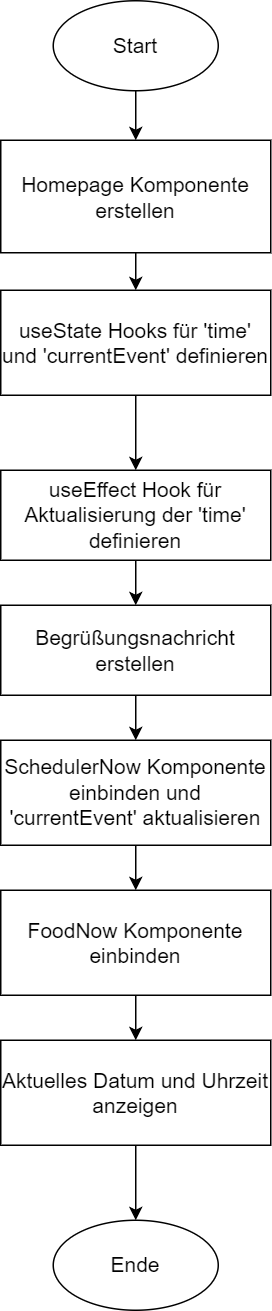
\includegraphics[height=0.5\textheight]{images/PAPHomepage}}
	\caption{PAP Homepage}
\end{figure}

\subsection{Food}
\subsubsection{Konzept}
Die Food-Komponente der DHBW Star-Webseite ist ein wichtiger Teil der Anwendung,die Speisepläne anzeigt.
Die Daten werden von einer Mensa-APi abgerufen die in einem Docker-Container erstellt wird. Dieser Vorgang wird in dem Kapitel Docker näher beschrieben.
Der Default-Speiseplan ist immer der aktuelle Tag, zu dem werden für die nächsten zehn Tage die Speisepläne angezeigt. Außer an Wochenenden, da ist die Mensa geschlossen.
Der ursprüngliche Plan war, die \emph{OpenMensa} API zu verwenden. Diese API bietet eine umfassende und benutzerfreundliche Schnittstelle zum Abrufen von Mensa-Daten. Besonders reizvoll war die Tatsache, dass  Daten für eine Vielzahl von Kantinen bereitgestellt werden, darunter auch für die Kantine Erzbergerstraße.\cite{openmensa}
Allerdings stellt sich heraus, dass die Daten für die Mensa Erzbergerstraße nicht aktuell sind. Die neuesten verfügbaren Daten beziehen sich auf Juli 2022. Dies reicht für unsere Zwecke nicht aus, da wir aktuelle und genaue Daten benötigen.\cite{openmensa-canteen33}\\
Als Alternative wurde sich für die  KA-Mensa-API entschieden. Diese API liefert aktuellere und genauere Daten. Darüber hinaus wird ein Docker-Image mitgeliefert, sodass die API nahtlos in die bestehende Docker-Infrastruktur integriert werden kann.\cite{ka-mensa-api} \\
Da Docker bereits für andere Teile der Anwendung genutzt wird, ist die Integration der KA-Mensa API in die  bestehende Docker-Infrastruktur ein logischer und effizienter Schritt. Dadurch konnte die Food-Komponente der Website stets aktuelle und genaue Daten anzeigen, unterstützt durch die Docker-Technologie.
In diesem Programmablaufplan ist die Food-Komponente visuell erklärt.\\
\begin{figure}[htbp]
	\centering
	\fbox{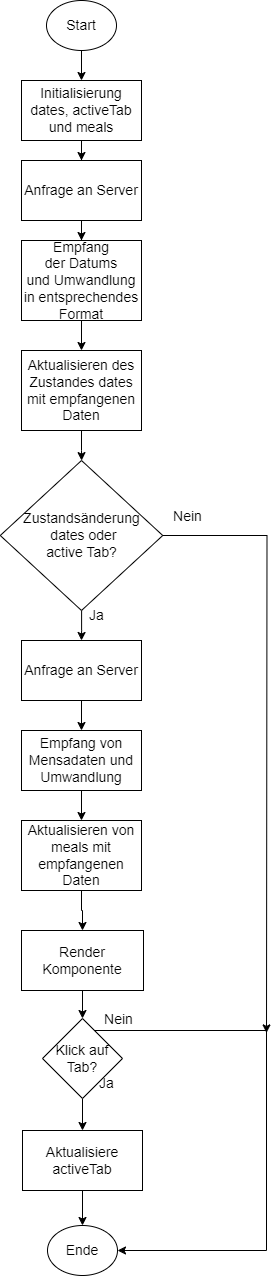
\includegraphics[height=0.65\textheight]{images/PAPFood}}
	\caption{PAP Food}
\end{figure}
\newpage
Zudem ist in der nächsten Abbildung die Webseite der Food-Komponente abgebildet.
\begin{figure}[htbp]
	\centering
	\fbox{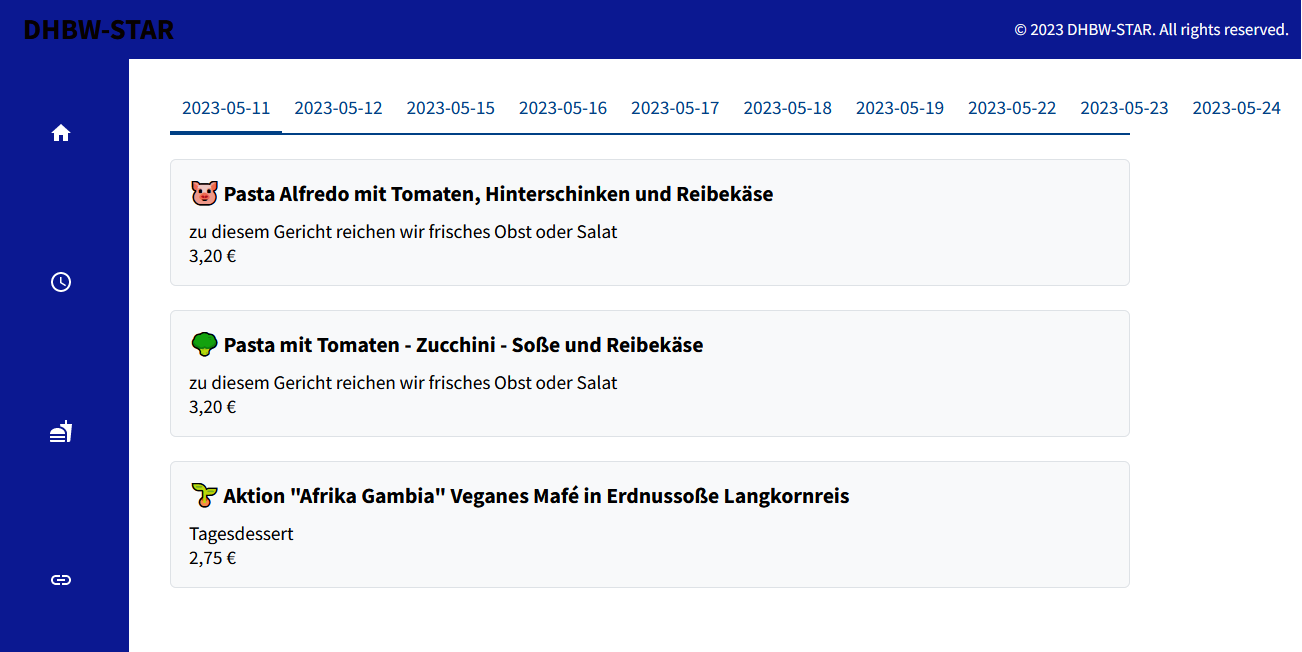
\includegraphics[height=0.3\textheight]{images/Food}}
	\caption{Food Website}
\end{figure}
\subsubsection{Implementierung}
Die Implementierung der Foodkomponente der DHBW Star-Webseite basiert auf der Verwendung grundlegender und erweiterter Funktionen der React- und \emph{Axios}-Bibliotheken zur Verarbeitung von HTTP-Anfragen.
Die \emph{Food}-Komponente wird als funktionelle Komponenten definiert und nutzt React-Hooks, um den internen Zustand und Nebenwirkungen zu verwalten. Mit dem Hook \emph{useState} werden drei Statusvariablen definiert: \emph{dates}, \emph{activeTab} und \emph{meals}. \emph{Dates} speichert  Daten, an denen Mahlzeiten verfügbar sind, \emph{activeTab} speichert den Index des aktuell ausgewählten Datums und \emph{Meals} speichert Mahlzeitinformationen für das aktuell ausgewählte Datum. Der \emph{useEffect}-Hook wird zweimal verwendet. Einmal, um das Datum abzurufen, an dem die Komponente zum ersten Mal gerendert wird, und einmal, um die Informationen zur Essenszeit abzurufen, wenn sich das aktive Datum ändert. Die Funktionen \emph{fetchDates} und \emph{fetchMeals} verwenden die \emph{Axios}-Bibliothek, um eine HTTP-GET-Anfrage an den Server zu senden, um Daten abzurufen. 
Informationen zu Mahlzeiten werden angezeigt, indem das Array \emph{Meals} durchlaufen und  für jede Mahlzeit ein JSX-Element generiert wird. Es verwendet die Funktion \emph{getEmoji}, um passende Emojis basierend auf Essensklassifikatoren zu generieren.\\
Dies ist der dazugehörige Code:
\newpage
\begin{lstlisting}[language=JavaScript,
	frame=single,           % Ein Rahmen um den Code
	framexleftmargin=15pt,  % Rahmen link von den Zahlen
	style=algoBericht,
	label={Food-Komponente},
	captionpos=b ,          % Caption unter den Code setzen
	caption={Food-Komponente}]
import React, { useState, useEffect } from "react";
import axios from "axios";
import "./Food.css";

const getEmoji = (classifier,name) => {
	/// Returns Emojis depending on the classifiers
};
const Food = () => {
  const [dates, setDates] = useState([]);
  const [activeTab, setActiveTab] = useState(0);
  const [meals, setMeals] = useState([]);
  
  useEffect(() => {
  	fetchDates();}, []);
  useEffect(() => {
   if (dates.length > 0) {
   	fetchMeals(dates[activeTab]);}
   }, [dates, activeTab]);
  const fetchDates = async () => {
  	try {
  	 const response = await axios.get(process.env.
  	 REACT_APP_MENSA_ADDRESS+"/plans");
  	 const dateList = response.data.data.map((date) =>
  	 `{date.date.year}-{(date.date.month + 1).toString()
  	 .padStart(2, "0")}-{date.date.day.toString()
  	 .padStart(2, "0")}`).slice(0, 10);
     setDates(dateList);} 
    catch (error) {
     console.error("Error fetching dates:", error);}
 };

const fetchMeals = async (date) => {
  try {
   const response = await axios.get(
   process.env.REACT_APP_MENSA_ADDRES-+
   `/plans/{date}?canteens=erzberger`);
   let mealData = response.data.data[0].lines
   .slice(0, 3).map((line) => ({
   	main: line.meals[0],
   	description: line.meals[1]?.name,}));
   if (!mealData[0]['main']){
   console.log("FEIERTAG")
   mealData=[{
   	main: {
   	 classifiers: 'Nein',
   	 name:"Feiertag/kein Essen",
   	 price:"0 Euro"},
    description: "An dem heutigen Tag ist 
    die Mensa geschlossen."}]}
   setMeals(mealData);
  } catch (error) {
  console.error("Error fetching meals:", error);
}};
return (
 <div className="mensa-plan">
 <div className="tabs">
 {dates.map((date, index) => (
  <button
    key={index}
    className={`tab {index === activeTab ? "active" : ""}`}
    onClick={() => setActiveTab(index)}>
    {date}</button>))}
  </div>
  <div className="tab-content">
  {meals.map((mealObj, index) => {
    const meal = mealObj.main;
    if (meal?.empty) {
     return (
     <div key={index} className="no-meal">
     <h3>Feiertag/Kein Essen</h3></div>);
 } else {
  return (
  <div key={index} className="meal">
  <h3>
  {getEmoji(meal.classifiers[0],meal.name)} {meal.name}
  </h3>
  <p>{mealObj.description}</p>
  <p>{meal.price}</p></div>);}})}
  </div>
  </div>);};

export default Food;
	
\end{lstlisting}

Die Implementierung der \emph{Food}-komponente wurde so konzipiert, dass Datenerfassung und -präsentation sauber getrennt werden. Mit React-Hooks ist es möglich den Komponentenstatus effizient zu verwalten und die Benutzeroberfläche automatisch zu aktualisieren, wenn sich der Status ändert. Die \emph{Axios}-Bibliothek macht die Bearbeitung von HTTP-Anfragen einfach und zuverlässig. Diese Struktur ermöglicht auch eine einfache Anpassung und Erweiterung der Komponente, wenn in Zukunft zusätzliche Funktionen oder Änderungen erforderlich sind.

\subsubsection{FoodNow}
Die \emph{FoodNow}-Komponente der DHBW-Star-Webseite wurde entwickelt, um Nutzern aktuelle Informationen zur Essensverfügbarkeit in der Mensa zur Verfügung zu stellen. Es wurde mithilfe der React- und Axios-Bibliotheken zur Verwaltung von HTTP-Anfragen implementiert. 
Diese Komponente besteht aus Funktionskomponenten, die mithilfe der \emph{useState}- und \emph{useEffect}-Hooks von React den Status verwalten und Nebenwirkungen behandeln. Es werden zwei Zustandsvariablen definiert. Das eine ist \emph{meals}, das die aktuell verfügbaren Mahlzeiten speichert, und das andere ist \emph{mensaStatus}, das den aktuellen Status des Restaurants speichert (geöffnet oder kurz vor der Eröffnung). 
Der \emph{useEffect}-Hook wird verwendet, um die \emph{fetchMeals}-Funktion auszulösen, sobald die Komponente in der Benutzeroberfläche gerendert wird. Diese Funktion ruft zunächst die Funktion \emph{isMensaOpen} auf, um zu sehen, ob die Mensa geöffnet ist oder kurz vor der Eröffnung steht. Diese Funktion überprüft das aktuelle Datum und die aktuelle Uhrzeit und vergleicht sie mit den  Öffnungs- und Schließzeiten des angegebenen Restaurants. 
Wenn die Mensa geöffnet ist oder kurz vor der Eröffnung steht, wird eine HTTP-GET-Anfrage an den Mensa-Server gesendet, um die verfügbaren Mahlzeiten für den  Tag abzurufen. Erhaltene Mahlzeiten werden  im Status \emph{meals} gespeichert und der Status der Mensa wird in \emph{mensaStatus} gespeichert. 
Die Rendermethode der Komponente prüft, ob die Cafeteria geöffnet ist oder kurz vor der Eröffnung steht und stellt die verfügbaren Mahlzeiten entsprechend dar oder zeigt eine Meldung an, dass die Cafeteria geschlossen ist oder kurz vor der Eröffnung steht. Die Implementierung der \emph{FoodNow}-Komponente auf diese Weise ermöglicht eine effiziente Handhabung von Statusänderungen und Nebenwirkungen und hält die Benutzeroberfläche auf dem neuesten Stand. Die Axios-Bibliothek erleichtert Komponenten das Senden und Empfangen von HTTP-Anfragen. Diese Implementierung trägt dazu bei, dass der Code sauber und  organisiert bleibt, wodurch er einfacher zu lesen und zu warten ist.
In diesem Codeblock befindet sich der dazugehörige Code:
\begin{lstlisting}[language=JavaScript,
	frame=single,           % Ein Rahmen um den Code
	framexleftmargin=15pt,  % Rahmen link von den Zahlen
	style=algoBericht,
	label={FoodNow-Komponente},
	captionpos=b ,          % Caption unter den Code setzen
	caption={FoodNow-Komponente}]
import React, { useState, useEffect } from "react";
import axios from "axios";
import "./Food.css";
const getEmoji = (classifier, name) => {
	switch (classifier) {
		
}};
const FoodNow = () => {
  const [meals, setMeals] = useState([]);
  const [mensaStatus, setMensaStatus] = 
  useState({ isOpen: false, isBeforeOpening: false });
  useEffect(() => {
    fetchMeals();}, []);
  const isMensaOpen = () => {
  	const now = new Date();
  	const day = now.getDay();
  	const time = now.getHours() * 60 + now.getMinutes();
  	const openingTime = 11 * 60 + 15;
  	const closingTime = 13 * 60 + 30;
  	const beforeOpening = time < openingTime;
  	 return {
  	  isOpen: day >= 1 && day <= 5 && time >= openingTime 
  	  && time <= closingTime,
  	  isBeforeOpening: beforeOpening,};};
    const fetchMeals = async () => {
     try {
      const mensaStatus = isMensaOpen();
      if (mensaStatus.isOpen || mensaStatus.isBeforeOpening) {
       const today = new Date().toISOString().slice(0, 10);
       const response = await axios.get(
       process.env.REACT_APP_MENSA_ADDRESS+
       `/plans/${today}?canteens=erzberger`);
       let mealData = response.data.data[0].lines.slice(0, 3)
       .map((line) => ({
       	main: line.meals[0],
       	description: line.meals[1]?.name,}));
       if (!mealData[0]["main"]) {
        console.log("FEIERTAG");
         mealData = [{
         	main: {
             classifiers: "Nein",
             name: "Feiertag/kein Essen",
             price: "0",},
           description: "An dem heutigen Tag ist 
            die Mensa geschlossen.",},];}
        setMeals(mealData);
        setMensaStatus(mensaStatus);
     } else {
      setMensaStatus({ isOpen: false, isBeforeOpening: false });}
      } catch (error) {
      console.error("Error fetching meals:", error);}};
  return (
   <div className="mensa-plan">
   <div className="tab-content">
   {mensaStatus.isOpen || mensaStatus.isBeforeOpening ? (
   	 meals.length > 0 ? (
   	 meals.map((mealObj, index) => {
   	  const meal = mealObj.main;
   	  return (
   	  <div key={index} className="meal">
   	  <h3>
   	  {getEmoji(meal.classifiers[0], meal.name)}{meal.name}
   	  </h3>
   	  <p>{mealObj.description}</p>
   	  <p>{meal.price}</p>
   	  </div>);})) : (
     <div className="no-meal">
     <h3>Keine Informationen fuer heute verfuegbar</h3>
     </div>)) : (
     <div className="no-meal">
     <h3>Die Mensa ist geschlossen</h3></div>)}
   {mensaStatus.isBeforeOpening && (
   	<div className="before-opening">
   	<h3>Die Mensa ist noch geschlossen. 
   	Sie oeffnet um 11:15 Uhr.</h3></div>)}
   </div>
   </div>);};
export default FoodNow;

\end{lstlisting}
\newpage
\subsection{Scheduler}
\subsubsection{Konzept}
Die \emph{Scheduler}-Komponente wurde entwickelt, um Nutzern einen Überblick über geplante Vorlesungen in der DHBW-Star-Webseite zu geben. Es wurde mithilfe der React-Bibliothek, der Axios-Bibliothek zum Verwalten der HTTP-Anfragen und der FullCalendar-Bibliothek zum Rendern der Ereignisse im Kalender implementiert.\\
Die Webseite der \emph{Scheduler}-Komponente ist in dieser Abbildung dargestellt.\\
\begin{figure}[htbp]
	\centering
	\fbox{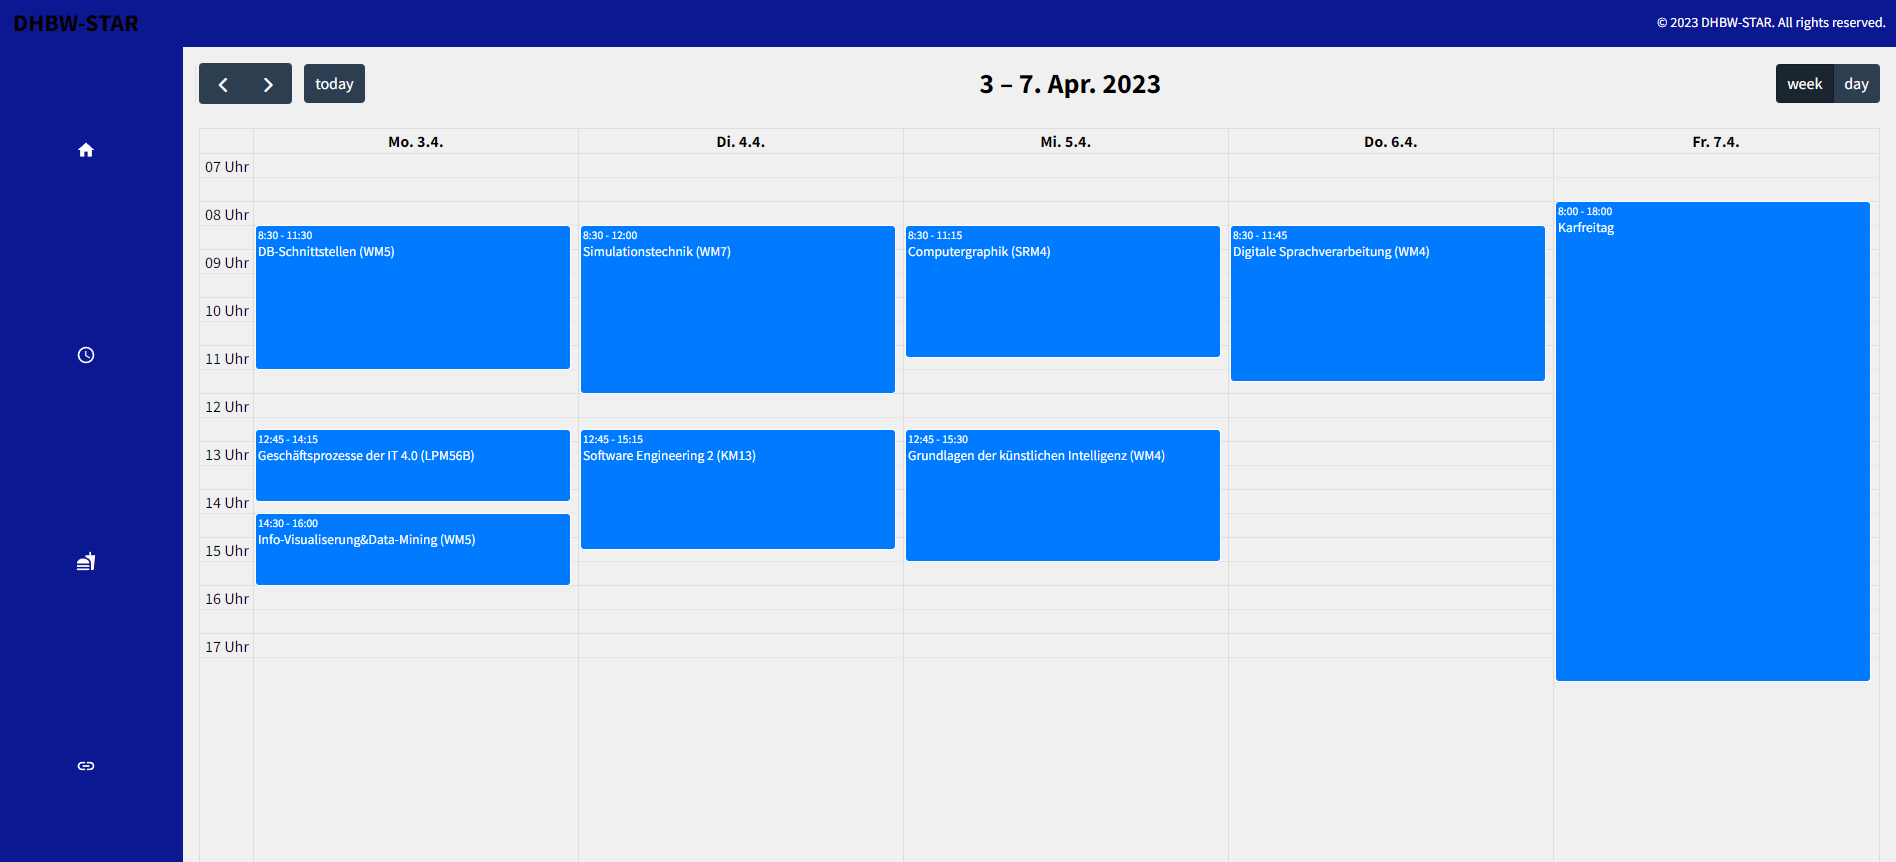
\includegraphics[height=0.35\textheight]{images/Scheduler}}
	\caption{Scheduler}
\end{figure}
\newpage
Die Grundschritte der Implementierung werden in diesem Programmablaufplans visualisiert um die Grundfunktion verständlicher zu machen.
\begin{figure}[htbp]
	\centering
	\fbox{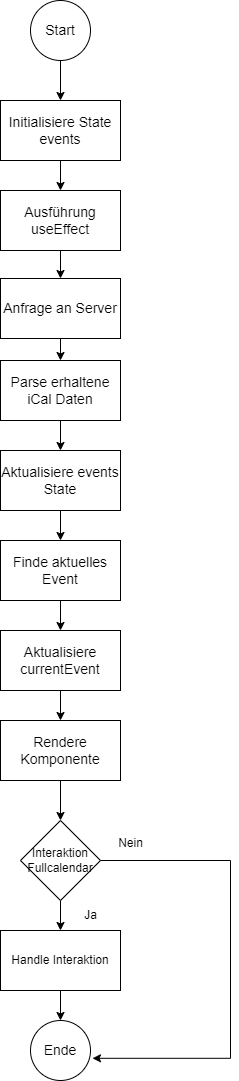
\includegraphics[height=0.65\textheight]{images/PAPScheduler}}
	\caption{PAP Scheduler}
\end{figure}
\newpage
\subsubsection{Implementierung}
Das ist der Code für die \emph{Scheduler}-Komponente:
\begin{lstlisting}[language=JavaScript,
	frame=single,           % Ein Rahmen um den Code
	framexleftmargin=15pt,  % Rahmen link von den Zahlen
	style=algoBericht,
	label={Scheduler-Komponente},
	captionpos=b ,          % Caption unter den Code setzen
	caption={Scheduler-Komponente}]
import React, { useState, useEffect } from 'react';
import axios from 'axios';
import FullCalendar from '@fullcalendar/react';
import dayGridPlugin from '@fullcalendar/daygrid';
import timeGridPlugin from '@fullcalendar/timegrid';
import interactionPlugin from '@fullcalendar/interaction';
import './Scheduler.css';
import ICAL from 'ical.js';
import '@fullcalendar/core/locales-all';
import { isWithinInterval } from 'date-fns';

const Scheduler = ({ setCurrentEvent }) => {
  const [events, setEvents] = useState([]);
  useEffect(() => {
   const fetchData = async () => {
   try {
    const response = await 
    axios.get(
    process.env.REACT_APP_PROXY_ADDRESS+'/schedule');
    const data = response.data;
    const parsedEvents = parseEvents(data);
    setEvents(parsedEvents);
    const currentEvent = getCurrentEvent(parsedEvents);
    setCurrentEvent(currentEvent);
} catch (error) {
  console.error(
  'Error fetching schedule data:', error);
   }}
  fetchData();}, [setCurrentEvent]);

 const getCurrentEvent = (events) => {
  const now = new Date();
  const currentEvent = events.find(
  (event) =>isWithinInterval(now, 
  { start: event.start, end: event.end }) &&
  now.getTime() <= event.end.getTime());
  return currentEvent;};

 const parseEvents = (icalData) => {
  const jcalData = ICAL.parse(icalData);
  const comp = new ICAL.Component(jcalData);
  const events = comp.getAllSubcomponents('vevent');
  const now = new Date();
  const startDate = ICAL.Time.fromJSDate(
  new Date(now.getFullYear() - 1, 
  now.getMonth(), now.getDate()));
  const endDate = ICAL.Time.fromJSDate(
  new Date(now.getFullYear() + 1, 
  now.getMonth(), now.getDate()));
  const parsedEvents = [];
  events.forEach(eventComponent => {
   const event = new ICAL.Event(eventComponent);
   const start = event.startDate;
   const end = event.endDate;
   if (event.isRecurring()) {
   	const iterator = event.iterator();
   	let next;
   	while ((next = iterator.next())) {
   	  if (next.compare(startDate) < 0) {
   	  	continue;}
      if (next.compare(endDate) > 0) {
      	break;}
      const duration = end.subtractDate(start);
      const eventStart = next;
      const eventEnd = eventStart.clone();
      eventEnd.addDuration(duration);
      parsedEvents.push({
       title: event.summary,
       start: eventStart.toJSDate(),
       end: eventEnd.toJSDate(),
       location: event.location ? 
       event.location.value : '',
       description: event.description,});}
   } else {
       parsedEvents.push({
        title: event.summary ,
        start: start.toJSDate(),
        end: end.toJSDate(),
        location: event.location,
        description: event.description,});}
});
 console.log(parsedEvents);
 return parsedEvents;};

return (
  <div className="scheduler">
  <FullCalendar
    plugins={[dayGridPlugin, timeGridPlugin, interactionPlugin]}
    initialView="timeGridWeek"
    headerToolbar={{
      left: 'prev,next today',
      center: 'title',
      right: 'timeGridWeek,timeGridDay',}}
    events={events}
    eventColor="#007bff" //// Blaue Akzente
    locale="de"
    allDaySlot={false} // Entfernt die Anzeige fuer "all day"-Events
    nowIndicator={true} 
    // Fuegt einen roten Zeitstrahl fuer die aktuelle Zeit hinzu
    weekends={false} // Versteckt Wochenenden
    slotMinTime="07:00:00" // Startzeit fuer Zeitslo-ts
    slotMaxTime="18:00:00" // Endzeit fuer Zeitslots/>
    </div>
    );
};
export default Scheduler;
\end{lstlisting}
\newpage
Die \emph{Scheduler}-Komponente besteht aus Funktionskomponenten, die die React-Hooks \emph{useState} und \emph{useEffect} verwenden, um den Status zu verwalten und Nebenwirkungen zu behandeln. Der \emph{useState}-Hook wird verwendet, um den Status des im Kalender angezeigten Ereignisses zu speichern,  und der \emph{useEffect}-Hook wird verwendet, um die \emph{fetchData}-Funktion auszulösen, sobald die Komponente in der Benutzeroberfläche angezeigt wird.\\
Die \emph{fetchData}-Funktion sendet eine HTTP-GET-Anfrage an den Server,um \emph{ical}-Daten für geplante Ereignisse abzurufen. Diese Daten werden dann mithilfe der \emph{parseEvents}-Funktion in ein Format konvertiert, das von der \emph{FullCalendar}-Bibliothek verstanden wird. Diese Funktion verwendet die \emph{ICAL.js}-Bibliothek, um die \emph{ical}-Daten zu analysieren und in ein JavaScript-Objekt zu konvertieren. Es berücksichtigt auch wiederkehrende Ereignisse und generiert für jede Wiederholung innerhalb eines bestimmten Zeitraums ein eigenes Ereignis.\\
Die Funktion \emph{getCurrentEvent} wird verwendet, um das aktuelle Ereignis abzurufen, also das Ereignis, das gerade auftritt. Diese durchsucht die Liste der Ereignisse nach Ereignissen, deren Start- und Endzeit das aktuelle Datum enthalten. Dieses Ereignis wird zur Anzeige durch eine andere Komponente in der Anwendung an die übergeordnete Komponente zurückgegeben.\\
Schließlich gibt die \emph{Scheduler}-Komponente eine \emph{FullCalendar}-Komponente zurück, die mit  entsprechenden Eigenschaften konfiguriert ist, um die Ereignisse benutzerfreundlich anzuzeigen.Die Komponente nutzt mehrere Plugins von FullCalendar, um unterschiedliche Ansichten und Interaktionen zu ermöglichen.\\
Diese Art und Weise der Implementierung bietet eine effiziente und flexible Möglichkeit, geplante Ereignisse anzuzeigen. Es stellt sicher, dass die Daten immer auf dem neuesten Stand sind und ermöglicht Benutzern eine einfache und intuitive Übersicht ihrer Veranstaltungen. Die Verwendung etablierter Bibliotheken wie \emph{Axios}, \emph{FullCalendar} und \emph{ICAL.js} reduziert die Codekomplexität und erhöht die Zuverlässigkeit und Wartbarkeit.
\subsubsection{Proxy-Server}
Der Proxy-Server ist so konzipiert, dass er die Cross-Origin Resource Sharing (CORS)-Richtlinie umgeht, die von APIs auferlegt werden. Cross-Origin Resource Sharing (CORS) ist eine Sicherheitsmaßnahme, die in modernen Webbrowsern implementiert ist. Der Zweck besteht darin, es zu ermöglichen, welche Webressourcen auf Daten in anderen Domänen zugreifen können zu steuern. Dies ist wichtig, um das Risiko von Cross-Site Request Forgery (CSRF) und anderen Arten von Angriffen zu verringern, die darauf abzielen, die Identität eines Benutzers zu kapern. Sie verhindern den Zugriff von einer Domäne (Ursprung) auf Ressourcen in einer anderen Domäne,sofern dies nicht ausdrücklich erlaubt ist \cite{ionos-de}.\\
In diesem speziellen Fall verfügt die API\\ \emph{http://rapla.dhbw-karlsruhe.de/rapla?page=iCalanduser=vollmerandfile=tinf20b3} über eine CORS-Richtlinie, die Clients den direkten Zugriff auf Kalenderdaten verbietet. Dies geschieht aus verschiedenen Gründen, unter anderem zum Schutz der Datenintegrität und zur Verhinderung bestimmter Arten von Angriffen\cite{crashtest-security-com}.\\
Bei dem Proxy-Server von DHBW-Star erscheint die Umgehung der CORS-Richtlinie gerechtfertigt und sinnvoll. Der Hauptgrund dafür ist, dass die Anwendung für ihre Funktion auf Daten der API\\ \emph{http://rapla.dhbw-karlsruhe.de/rapla?page=iCalanduser=vollmerandfile=tinf20b3} angewiesen ist. Wenn der direkte Zugriff auf diese Daten durch die CORS-Richtlinie der API verboten ist, kann die Anwendung  ihre Funktion nicht ausführen.\\
Ein weiterer wichtiger Faktor ist, dass die Umgehung der CORS-Richtlinie in diesem Fall auf sichere Weise durch die Verwendung eines Proxy-Servers erfolgen kann. Ein Proxyserver fungiert als Vermittler zwischen Clients und APIs und stellt sicher, dass  Daten auf sichere und kontrollierte Weise abgerufen werden. Dadurch wird das Risiko von Sicherheitsproblemen minimiert.\\
Dieses Bild veranschaulicht die Rolle des Proxy-Servers genauer.\\
\begin{figure}[htbp]
	\centering
	\fbox{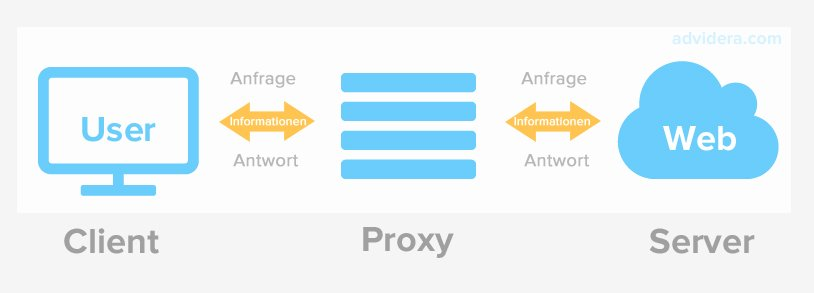
\includegraphics[height=0.25\textheight]{images/Proxyserver}}
	\caption{Proxy-Server}
\end{figure}

Der Proxy-Server wurde in \emph{Node.js} mithilfe des Express-Frameworks implementiert, das ein benutzerfreundliches Framework zum Erstellen von Webanwendungen und APIs bietet. Zudem wurde das CORS-Paket importiert, um \emph{Axios} zum Senden von HTTP-Anfragen an CORS-Funktionen und APIs bereitzustellen.\\
Ein Cache-Objekt wurde eingeführt, um  Antwortdaten für einen bestimmten Zeitraum (in diesem Fall 1 Stunde) zu speichern und unnötige Anfragen an die API zu vermeiden. Diese Cache-Implementierung trägt dazu bei, die API-Last zu reduzieren und die Anwendungsleistung zu verbessern, indem  die Anzahl der an die API gesendeten Anforderungen reduziert wird. Wenn die Anfrage innerhalb des Cache-Zeitraums wiederholt wird, werden die zwischengespeicherten Daten an den Client gesendet, ohne erneut auf die API zuzugreifen.\\
Die Proxy-Anwendung stellt einen einzelnen Endpunkt \emph{/schedule} bereit, um Kalenderdaten auf Anfrage asynchron abzurufen. Zunächst prüft es, ob sich die Daten im Cache befinden und innerhalb des Cache-Zeitraums noch  gültig sind. Falls vorhanden, werden die zwischengespeicherten Daten an den Client gesendet. Andernfalls wird eine Anfrage an die API gesendet, um die neuesten Kalenderdaten abzurufen.Antwortdaten werden zwischengespeichert und an den Client gesendet.\\
Der Proxy-Server läuft auf Port 3002 oder einem anderen Port, der durch die Umgebungsvariable \emph{PROXYPORT} angegeben wird. Der Proxy-Server ermöglicht es der Scheduler-Anwendung, CORS-Richtlinien zu umgehen und auf die Kalenderdaten der API zuzugreifen, um sie im Client darzustellen.\
Dies ist der zu entsprechende Code:
\begin{lstlisting}[language=JavaScript,
	frame=single,           % Ein Rahmen um den Code
	framexleftmargin=15pt,  % Rahmen link von den Zahlen
	style=algoBericht,
	label={Proxy-Server},
	captionpos=b ,          % Caption unter den Code setzen
	caption={Proxy-Server}]
const express = require('express');
const cors = require('cors');
const axios = require('axios');
const cach = {}
const cachDuration = 3600000; //1h
const kurs = 'tinf20b3'
const app = express();
app.use(cors());
app.get('/schedule', async (req, res) => {
 if (kurs in cach && cach['tinf20b3']
 .time > new Date().getTime())
 { console.log("Get cached Data");
 res.send(cach['tinf20b3'].data);}
 else{
  try {
   const response = await axios.get(
   'http://rapla.dhbw-karlsruhe.de/rapla?
   page=iCal&user=vollmer&file=tinf20b3');
   cach[kurs] = {
    time: new Date().getTime() + cachDuration,
    data: response.data};
    console.log("save Data in cache:" + cach['tinf20b3'].time);
    res.send(response.data);} 
   catch (error) {res.status(500).send({ error: 
   	'An error occurred while fetching the data.' });}}});
   const PORT = process.env.PROXY_PORT || 3002;

app.listen(PORT, () => console.log(`Proxy 
server running on port ${PORT}`));
	
\end{lstlisting}
\subsubsection{SchedulerNow}
Die Komponente \emph{SchedulerNow} ist eine spezielle Komponente, die entwickelt wurde, um  aktuelle Ereignisse (z. B. laufende Vorlesungen) aus dem iCalendar-Format (iCal) zu extrahieren und anzuzeigen. Diese Komponente ist in React geschrieben und verwendet \emph{useState}- und \emph{useEffect}-Hooks, um den internen Status zu verwalten. Dieser Code entspricht der \emph{SchedulerNow}-Komponente:

\begin{lstlisting}[language=JavaScript,
	frame=single,           % Ein Rahmen um den Code
	framexleftmargin=15pt,  % Rahmen link von den Zahlen
	style=algoBericht,
	label={SchedulerNow-Komponente},
	captionpos=b ,          % Caption unter den Code setzen
	caption={SchedulerNow-Komponente}]
import React, { useState, useEffect } from 'react';
import axios from 'axios';
import ICAL from 'ical.js';
import { isWithinInterval } from 'date-fns';
import './SchedulerNow.css';

const SchedulerNow = () => {
  const [currentEvent, setCurrentEvent] = useState(null);
  useEffect(() => {
   const fetchData = async () => {
   	try {
   	 const response = await axios.get(process.env.
   	 REACT_APP_PROXY_ADDRESS+'/schedule');
   	 const data = response.data;
   	 const parsedEvents = parseEvents(data);
   	 const currentEvent = getCurrentEvent(parsedEvents);
   	 setCurrentEvent(currentEvent);
  } catch (error) {
    console.error('Error fetching schedule data:', error);}
 };
  fetchData();}, []);
 const getCurrentEvent = (events) => {
  const now = new Date();
  const currentEvent = events.find(
  (event) => isWithinInterval(now, 
  { start: event.start, end: event.end }));
  return currentEvent;};
  const parseEvents = (icalData) => {
  	const jcalData = ICAL.parse(icalData);
  	const comp = new ICAL.Component(jcalData);
  	const events = comp.getAllSubcomponents('vevent');
  	const now = new Date();
  	const startDate = ICAL.Time.fromJSDate(new Date(
  	now.getFullYear(), now.getMonth()-1, now.getDate()));
  	const endDate = ICAL.Time.fromJSDate(new Date(
  	now.getFullYear() + 1, now.getMonth(), now.getDate()));
  	const parsedEvents = [];
  	events.forEach(eventComponent => {
  	 const event = new ICAL.Event(eventComponent);
  	 const start = event.startDate;
  	 const end = event.endDate;
  	 if (event.isRecurring()) {
  	  const iterator = event.iterator();
  	  let next;
  	   while ((next = iterator.next())) {
  	   	if (next.compare(startDate) < 0) {
  	   	  continue;}
     	if (next.compare(endDate) > 0) {
     	  break;}
       const duration = end.subtractDate(start);
       const eventStart = next;
       const eventEnd = eventStart.clone();
       eventEnd.addDuration(duration);
       parsedEvents.push({
       	title: event.summary,
       	start: eventStart.toJSDate(),
       	end: eventEnd.toJSDate(),
       	location: event.location ? event.location.value : '',
       	description: event.description,});}
       } else {
       parsedEvents.push({
       	title: event.summary ,
       	start: start.toJSDate(),
       	end: end.toJSDate(),
       	location: event.location,
       	description: event.description,});}});
       console.log('Parsed events:', parsedEvents);
       return parsedEvents;};
   
   const renderCurrentEvent = () => {
   	console.log('Current event:', currentEvent);
   	if (!currentEvent) {
   	  return <div className="no-lecture">Keine Vorlesung</div>;}
     
  return (
   <div className="current-lecture">
   <div className="title">{currentEvent.title}</div>
   {currentEvent.location && (
   	<div className="location">{currentEvent.location}</div>)}
   </div>);
    };
 
 return (
 <div className="scheduler-now">
 {renderCurrentEvent()}</div>);};

export default SchedulerNow;
\end{lstlisting}

Zunächst wird der Zustand \emph{currentEvent} initialisiert, der das aktuelle Ereignis darstellt. Dieser Status wird später aktualisiert, wenn Daten von der API abgerufen und verarbeitet werden. 
Der \emph{useEffect}-Hook wird verwendet, um die \emph{fetchData}-Funktion aufzurufen, nachdem die Komponente gerendert wurde. \emph{fetchData} verwendet die \emph{Axios}-Bibliothek, um eine HTTP-GET-Anfrage an den Proxy-Server zu senden, um die iCal-Daten abzurufen. Diese asynchrone Funktion verwendet \emph{Try/Catch}, um  Fehler zu behandeln, die beim Abfragen der Daten auftreten können. Mit der Funktion \emph{parseEvents} werden \emph{iCal}-Daten in ein für JavaScript geeignetes Format konvertiert. Die \emph{ICAL.js}-Bibliothek wird verwendet,um\emph{iCal}-Daten zu analysieren und  Ereignisse zu extrahieren. Es berücksichtigt auch wiederkehrende Ereignisse und erstellt  für jede Wiederholung innerhalb des angegebenen Zeitraums ein separates Ereignis. 
Die Funktion \emph{getCurrentEvent} findet das aktuelle Ereignis, indem diese das aktuelle Datum und die aktuelle Uhrzeit mit den Start- und Endzeiten jedes Ereignisses vergleicht. Das ermittelte Ereignis wird  im Zustand gespeichert.Die Funktion \emph{renderCurrentEvent} ist für das Rendern des aktuellen Ereignisses verantwortlich. Diese prüft, ob es aktuelle Veranstaltungen gibt und zeigt eine Meldung an, dass keine Vorträge stattfinden bzw. die aktuellen Veranstaltungsdetails entsprechend. 

Diese Implementierung ermöglicht eine effiziente und reaktive Darstellung aktueller Ereignisse. Durch die Verwendung des React-Frameworks zum asynchronen Abrufen von Daten können Komponenten schnell auf Änderungen reagieren und aktuelle Ereignisse zeitnah aktualisieren. Ein Proxy-Server ermöglicht es Komponenten, CORS-Richtlinien zu umgehen und gleichzeitig die  Haupt-API auszulagern. Durch die Verwendung von Caching-Techniken und das Parsen von \emph{iCal}-Daten in Ihrer Clientanwendung wird die Leistung weiter optimiert und die Skalierbarkeit verbessert.
\newpage
\subsection{Links}
\subsubsection{Konzept}
Die \emph{Link}-Komponente von React ist eine spezielle Komponente, die dazu dient, eine Sammlung von Links zu verschiedenen Ressourcen anzuzeigen. Diese Komponente verwendet die \emph{useState}- und \emph{useEffect}-Hooks von React, um den internen Status zu verwalten und Effekte zu behandeln.
In den folgenden Abbildungen befinden sich die Webseite von der Links-Komponente und der Programmablaufplan
\begin{figure}[htbp]
	\centering
	\fbox{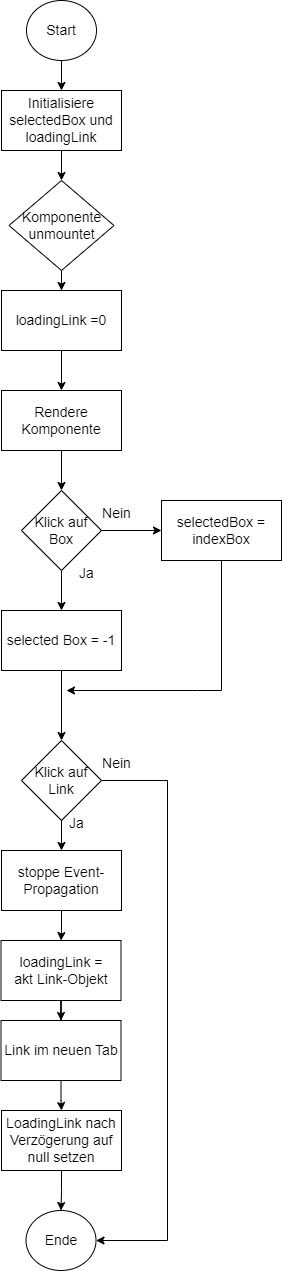
\includegraphics[height=0.7\textheight]{images/PAPLinks}}
	\caption{PAP Links}
\end{figure}
\begin{figure}[htbp]
	\centering
	\fbox{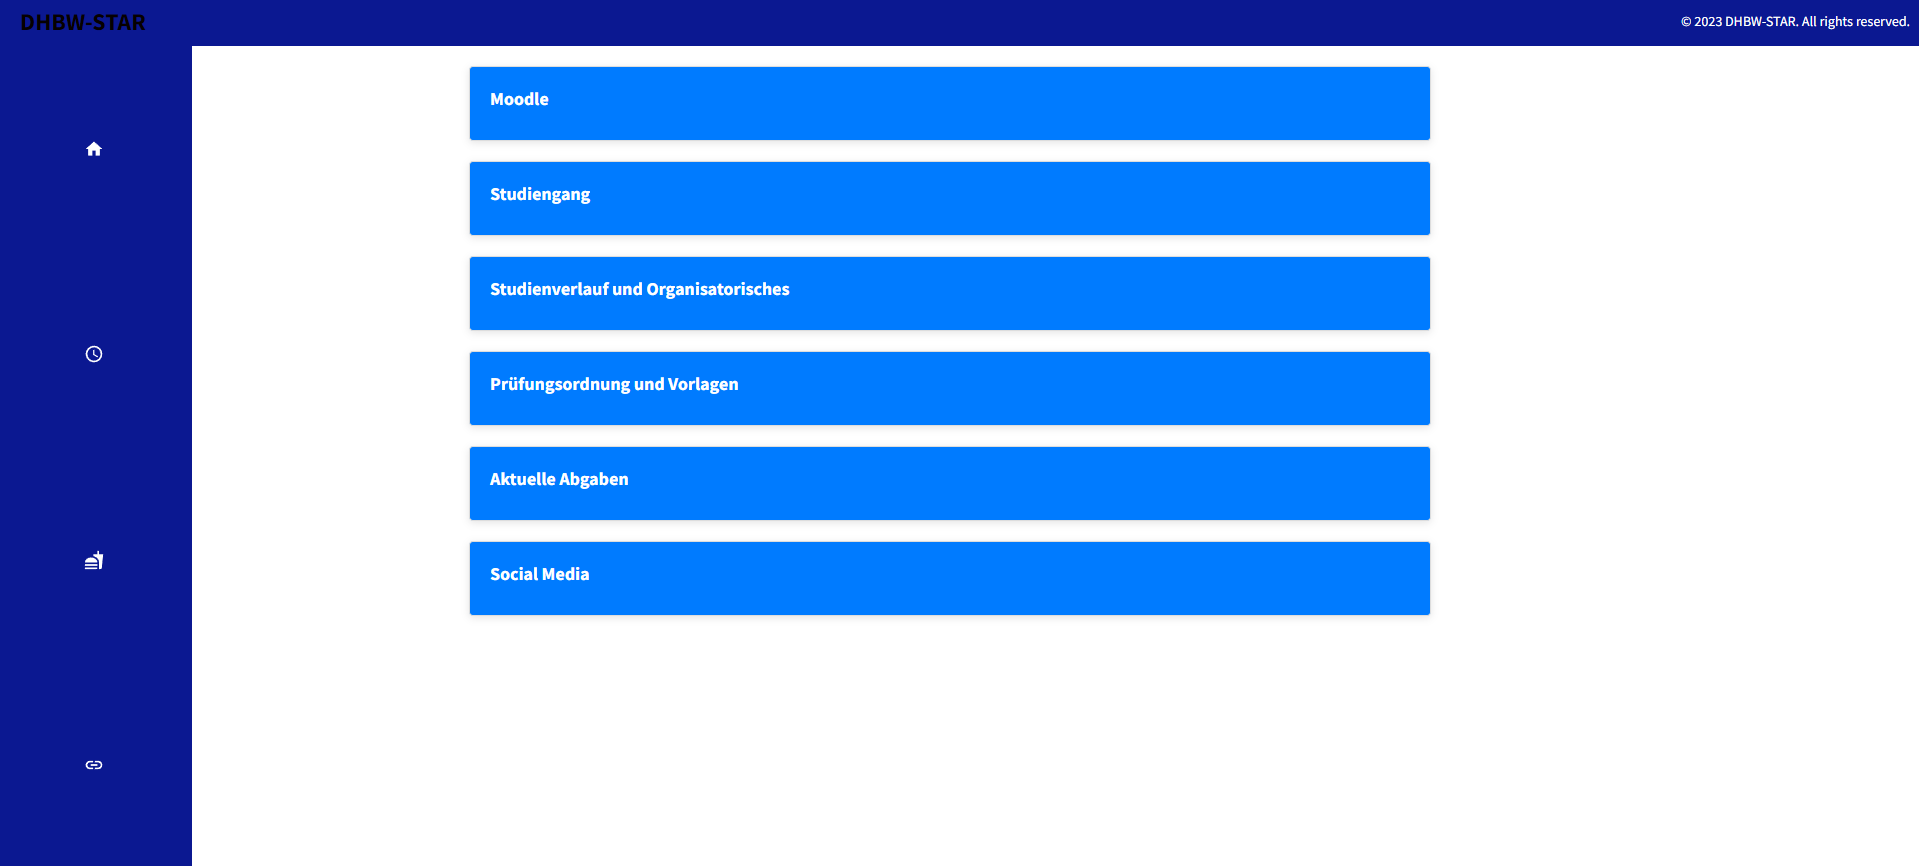
\includegraphics[height=0.3\textheight]{images/Links}}
	\caption{Links-Website}
\end{figure}
\newpage
\subsubsection{Implementierung}
Die Komponente \emph{Links} definiert zunächst eine Array-Struktur \emph{links}, die die verschiedenen Kategorien von Links und die jeweiligen Linkobjekte selbst enthält. Jedes Linkobjekt besteht aus einem Titel und einer URL.  
Der \emph{useState}-Hook wird verwendet, um zwei interne Zustandsvariablen zu definieren. \emph{selectedBox} verfolgt, welches Linkfeld gerade ausgewählt ist, und \emph{loadingLink} verfolgt, welcher Link gerade geladen wird.\\  
Der \emph{useEffect}-Hook wird verwendet, um den Status \emph{loadingLink} zurückzusetzen, wenn die Komponente nicht zusammengebaut ist. Hierbei handelt es sich um eine Sicherheitsmaßnahme, um sicherzustellen, dass der Status korrekt zurückgesetzt wird und es nicht zu unerwarteten Statusänderungen kommt, wenn Komponenten in  Zukunft wieder zusammengebaut werden. Die Funktion \emph{handleBoxClick} wird verwendet, um den Status der \emph{selectedBox} zu aktualisieren, wenn auf die Box geklickt wird. Durch erneutes Auswählen eines bereits ausgewählten Felds wird dessen Auswahl aufgehoben (d. h. \emph{selectedBox} wird auf -1 gesetzt). \\
Die Funktion \emph{handleLinkClick} dient zur Steuerung des Link-Klickverhaltens. Dadurch wird verhindert, dass das Standardereignisverhalten den Status \emph{loadingLink} aktualisiert und den Link in einem neuen Tab öffnet. Anschließend wird nach einer Verzögerung von 2000 ms der Status \emph{loadingLink} zurückgesetzt.  Die Rendermethode der Komponente durchläuft das Array \emph{links} und erstellt ein Element für jedes Feld und die darin enthaltenen Links. CSS-Klassen für  Boxen und Links werden basierend auf ihrem aktuellen Status dynamisch generiert.\\
Dies ist der zusammenhängende Code der Link-Komponente:
\begin{lstlisting}[language=JavaScript,
	frame=single,           % Ein Rahmen um den Code
	framexleftmargin=15pt,  % Rahmen link von den Zahlen
	style=algoBericht,
	label={Links-Komponente},
	captionpos=b ,          % Caption unter den Code setzen
	caption={Links-Komponente}]
import React, { useState,useEffect } from "react";
import "./Link.css";
const Link = () => {
 const links = [
 {
   \\ Ein Haufen Links die fuers Studieren wichtig sind.
    \\........................................
 }];

 useEffect(() => {
  return () => {
   setLoadingLink(null); // Setzt den Ladezustand zurueck, 
   wenn die Komponente unmountet wird};}, []);
   const [selectedBox, setSelectedBox] = useState(-1);
   const [loadingLink, setLoadingLink] = useState(null); 
   // Initialer State zu null
   const handleBoxClick = (index) => {
   if (selectedBox === index) {
   	setSelectedBox(-1);} 
   else {
   	setSelectedBox(index);}};
	const handleLinkClick = (e, boxIndex, linkIndex, link) => {
	  e.stopPropagation();
	  setLoadingLink({ boxIndex, linkIndex }); 
	  // Setzt den Lade-Link auf das aktuelle Link-Objekt
	  window.open(link.url, "_blank");
	  setTimeout(() => {
	   setLoadingLink(null); // Setzt den Lade-Link 
	   nach einer Verzoegerung zurueck
       }, 2000);};
   
  return (
  <div className="link-collection">
  {links.map((box, boxIndex) => (
  	<div key={boxIndex}
  	className={`link-box ${selectedBox === boxIndex ? 
  	"expanded" : ""}`}
    onClick={() => handleBoxClick(boxIndex)}>
      <h3>{box.title}</h3>
      <ul>
      {box.items.map((link, linkIndex) => (
       <li key={linkIndex}>
       <a className={loadingLink && 
       	loadingLink.boxIndex === boxIndex && 
       	loadingLink.linkIndex === linkIndex 
       	? "loading" : ""}
       onClick={(e) => handleLinkClick(
       	e, boxIndex, linkIndex, link)}>
       {link.title}
       </a></li>))}
      </ul>
      </div>))}
	</div>);
};
export default Link;

\end{lstlisting}

Die Implementierung dieser Komponente ermöglicht eine bequeme und effiziente Darstellung von Linkgruppen. Die Struktur und das Verhalten der Komponenten sind klar und intuitiv, und der Einsatz von Statusverwaltung und Event-Handlern stellt sicher, dass die Komponenten korrekt auf Benutzerinteraktionen reagieren und  aktualisiert werden. Durch die Verwendung von React für diese Komponente ist sie wiederverwendbar und lässt sich leicht in andere Teile einer größeren Anwendung integrieren.
\newpage
\section{Zusammenfassung}
DHBW-Star ist ein  neues Webportal-Angebot für Studierende der DHBW Karlsruhe. Es wurde  entwickelt, um einen zentralen, benutzerfreundlichen Zugangspunkt zu allen relevanten Ressourcen und Informationen bereitzustellen. Das Portal vereint die drei Hauptkomponenten Stundenplan, Essensplan und Linksammlung und ist auf die spezifischen Bedürfnisse der Studierenden zugeschnitten. 
Um sicherzustellen, dass DHBW-Star den tatsächlichen Bedürfnissen der Studierenden entspricht und einen echten Mehrwert bietet, haben wir eine Umfrage durchgeführt, um Feedback und Verbesserungsvorschläge zu sammeln.
Diese Umfrage wird in den nächsten zwei Kapiteln erklärt und ausgewertet.
\newpage
\section{Docker}

Damit die React App vom System unabhängig funktioniert, läuft sie in einem Docker Container. Dadurch werden Probleme mit unterschiedlichen Programmversionen und Konfigurationen verhindert.
Da die geplante Mensa API nicht funktioniert, wird als Alternative ein Container verwendet, der die Mensa API lokal bereitstellt.

\subsection{Die Dockerfile, compose.yaml und .env Dateien}

Für den React Containers wird ein Dockerfile Datei benötigt. In dieser wird beschrieben wie der Container zusammengebaut wird. Ein neuer Container kann auf vorhanden aufbauen oder komplett neu erstellt werden.

\begin{lstlisting}[language=vhdl,
	frame=single,           % Ein Rahmen um den Code
	framexleftmargin=15pt,  % Rahmen link von den Zahlen
	style=algoBericht,
	label={Dockerfile},
	captionpos=b           % Caption unter den Code setzen
	caption={Dockerfile für DHBW-Star}]
	FROM node:current-alpine
	
	RUN mkdir /reactApp
	WORKDIR /reactApp
	
	# Install React and dependencies
	COPY . .
	RUN npm init -y
	RUN npm install express cors axios
	RUN npm install
	RUN npm install ical.js
	RUN npm install -D concurrently
	RUN yarn build
	
	# Start both React app and proxy server
	CMD ["npm", "run", "start:all"]
\end{lstlisting}

Für DHBD Star wird der node Container von Dockerhub.com als Basis verwendet. Dieser besteht aus \emph{alpine}, einem minimalistischen Betriebssystem und NoteJS welcher für React benötigt wird.
Mit \emph{COPY} werden die Dateien des Projekts in den Container kopiert und mit \emph{RUN npm init} und \emph{RUN npm install} werden die benötigten Pakete für NoteJS installiert.
Zum Schluss wird mit \emph{RUN yarn build} das React Projekt gebaut und mit \emph{CMD ["npm", "run", "start:all"]} React und der Proxy gestartet. Der \emph{CMD} befehlt wird beim erstellen eines Container aus dem Image, immer ausgeführt. 

Damit die Mensa API und React zusammen starten, wird die \emph{compose.yaml} Datei und Docker compose verwendet.

\begin{lstlisting}[language=vhdl,
	frame=single,           % Ein Rahmen um den Code
	framexleftmargin=15pt,  % Rahmen link von den Zahlen
	style=algoBericht,
	label={Dockerfile},
	captionpos=b           % Caption unter den Code setzen
	caption={compose.yaml für DHBW-Star}]
	version: '3.9'
	services:
	react-app:
	build:
	dockerfile: ./Dockerfile
	tags:
	- "react:latest"
	ports:
	- "3003:3003"
	- "3002:3002"
	volumes:
	- ./src:/reactApp/src:ro
	- ./proxy-server.js:/reactApp/proxy-server.js:ro
	- ./.env:/reactApp/.env:ro
	mensa-api:
	image: meyfa/ka-mensa-api
	ports:
	- "3001:8080"
	environment:
	- MENSA_CORS_ALLOWORIGIN=*
\end{lstlisting}

Für den Service \emph{react-app} (DHBW Star) wird mit \emph{build} die oben beschrieben Dockerfiel Datei angeben. Somit baut der Befehl \emph{docker compose --build} ein neue Image mit dem React Projekt.
Der \emph{tags} gibt dem Container einen eindeutigen Namen.
Mit \emph{ports} werden die Ports vom Proxy(3002) und React (3003) nach außen frei gegeben.
Damit bei kleineren Änderungen im Projekt nicht immer ein neues Image erstellt werden muss, wird mit \emph{volums} die Projektdateien in den laufenden Container eingebunden.
Für die \emph{mensa-api} wird noch die Umgebungsvariable \emph{MENSA\_CORS\_ALLOWORIGIN=*} definiert.

Um die Container an unterschiedliche Gegebenheiten des Systems anpassen zu können, ohne etwas am React Projekt ändern zu müssen, bietet docer compose die Möglichkeit Umgebungsvariablen aus einer \emph{.env} Datei heraus zu definieren.
Da diese nicht teil von git sein sollte, wird eine \emph{.env\_template} angelegt. In dies stehen sind die verwendeten Umgebungsvariable mit Beispielen drin.
React verlangt für alle Umgebungsvariablen, die in der App zur Verfügung stehen sollen, dass sie mit \emph{REACT\_APP\_} beginnen.

\begin{lstlisting}[language=vhdl,
	frame=single,           % Ein Rahmen um den Code
	framexleftmargin=15pt,  % Rahmen link von den Zahlen
	style=algoBericht,
	label={Dockerfile},
	captionpos=b           % Caption unter den Code setzen
	caption={.env für DHBW-Star}]
	REACT_APP_MENSA_ADDRESS=http://localhost:3001 
	REACT_APP_PROXY_ADDRESS=http://localhost:3002
	PROXY_PORT=3002
	PORT=3003
\end{lstlisting}

\emph{REACT\_APP\_MENSA\_ADDRESS} und \emph{REACT\_APP\_PROXY\_ADDRESS} sind die Adressen der Services. Dies müssen mit der in \emph{compose.yaml} definierten Ports übereinstimmen. 

\section{Webserver}
Damit das Projekt auch über das Internet erreichbar ist, wird ein Root-Webserver mit einer Domain Adresse verwendet. Auf diesem ist bereits Docker, Nginx und Certbot Installiert.
Per github.com wird das Projekt auf den Server kopiert und die \emph{.env} Datei angepasst. Die Ports bleiben die Selben, nur das \emph{localhost} wird durch die Subdomains \emph{mensa.Domain} für den Mensa Container und \emph{ical.Domain} für den Proxy ersetzt.

Damit die Container unter ihrer Subdomain erreichbar sind, müssen diese in der Nginx Konfiguriert werden. In der Datei \emph{.../sites-enabled/star.conf} wird für jeden Service mit \emph{proxy\_pass} eine Weiterleitung eingerichtet.
Da auf dem Server bereits andere Webdienst laufen, ist Startseite unter der Subdomain \emph{star.Domain} erreichbar. Mit \emph{Certbot} werden noch SSL Zertifikate für alle Subdomains erstellt und automatisch eingerichtet.

Nach dem Neustart von Nginx, steht DHBW Star für alle Tester zur Verfügung.


\chapter{Umfrage/Datenerhebung}
Um eine Aussage über die Qualität der Webseite treffen zu können, wird eine Umfrage erstellt. In dieser sollen die Studenten, DHBW-Star mit den offiziellen Webseiten vergleichen und bewerten. Aus den Ergebnissen sollen Schlussfolgerungen zum Design von DHBW-Star gezogen werden und Vorschläge für Verbesserungen des Informationsangebotes der DHBW folgen.
Aus den Ergebnissen sollen Schlussfolgerungen zum Design von DHBW-Star gezogen werden und Vorschläge für Verbesserungen des Informationsangebotes der DHBW folgen.

\section{Vorbereitung}
Um eine aussagekräftige Umfrage erstellen zu können, müssen vorher folgende Überlegungen angestellt werden: \\
Was soll durch den Fragebogen gemessen werden? \\
Wer sind die Zielpersonen? \\
Welche Art von Fragen sind dafür geeignet? \\
Erst wenn diese Fragen geklärt sind, kann der Fragebogen erarbeitet werden.

Die ersten beiden Fragen sind von vorneherein klar:
Antwort: Ob DHBW-Star den Studenten besser gefällt als die offiziellen Websites.
Zielpersonen sind alle Teilnehmer im Tinf20B3 Kurs, da DHBW-Star für sie entworfen und designt wurde.

Die Entscheidung der Fragen-Art fällt auf eine Mischung von Messskala und Freitext. Es soll erst gemessen werten wie DHBW-Star im Vergleich zu den offiziellen Webseiten gefällt und der Freitext die Möglichkeit geben, zu beschreiben was besser oder schlechter gefallen hat.
Dabei werden alle Elemente der Seite zunächst einzeln Bewertet und danach die gesamte Website.
Zuletzt wird noch nach weiteren Verbesserungen und fehlenden Features gefragt.
Bei der Formulierung der Fragen werden die Checklisten von K. Wolfgang Kallus verwendet.
\cite{fragebogenKallus}(S. 142 + 143)

Diese beschreiben verschieden Kriterien für die Fragen um sicherzustellen, dass sie aussagekräftige Antworten liefern.

Um die Hürde für die Teilnahme und den Aufwand der Auswertung gering zu halten, wird die Umfrage online durchgeführt.

\section{Umfrage erstellen}
Um die Umfrage zu erstellen, wird die Webseite \emph{www.surveymonkey.de} verwendet. Die Entscheidung für diese Webseite fiel auf Grund der deutsche Top-Level-Domain und wegen ihrer Benutzerfreundlichkeit und Intuitivität, die es auch Menschen ohne technischen Hintergrund ermöglicht, Umfragen zu erstellen und zu verwalten \cite{surveymonkey-create-surveys}.

Die Plattform bietet eine Reihe von Funktionen, die das Erstellen und Verwalten von Umfragen erleichtern. Dazu gehören die Möglichkeit, Fragen zu gruppieren, um die Umfragestruktur klar und logisch zu gestalten, sowie Optionen, erste Umfragefragen so zu gestalten, dass sie die Befragten nicht verunsichern \cite{surveymonkey-create-surveys}.

Darüber hinaus bietet die Plattform auch Unterstützung bei der Umfrageauswertung. Es bietet Tools zur Datenanalyse und Präsentation von Ergebnissen und hilft dabei, die wichtigsten Botschaften aus Daten zu identifizieren und zu kommunizieren \cite{surveymonkey-auswertung-einer-umfrage}.

Schließlich bietet SurveyMonkey auch die Möglichkeit anonyme Antworten zu aktivieren. Dies ist besonders nützlich, wenn die Vertraulichkeit der Befragten wichtig ist \cite{surveymonkey-anonymous-responses}.

Testumfragen zu erstellen und aus erster Hand zu erfahren, wie Umfragen erstellt und ausgewertet werden, ist ebenfalls ein großer Vorteil von SurveyMonkey, da es möglich ist die Umfrage vor der endgültigen Veröffentlichung verfeinern und verbessern zu können. 
Mit dem kostenfreien Angebot können sich Umfragen bis zu zehn Fragen/Items erstellen. Es können allerdings auch maximal nur zehn Antworten ausgewertet werden. Was leider erst im Nachhinein aufgefallen ist.\\
Nach einem ersten Versuch wurde das kostenlose Angebot als ausreichend für diese Umfrage empfunden.
\\
Danach folgt der endgültige Fragebogen. Er besteht aus den folgenden 10 Fragen:
\begin{itemize}
	\item[01] {\emph{Frage}: Wie oft hast du DHBW-Star in den letzten 7 Tagen benutzt?\\
		\emph{Antwortmöglichkeiten}: kein mal, 1 mal, Mehr mal oder Täglich}
	\item[02]{\emph{F}:Auf welchem Gerät hast du DHBW-Star benutzt?\\
		\emph{AM}: PC, Tablet und Mobile}
	\item[03]{\emph{F}: Wie nützlich findest du die Startseite?\\
		\emph{AM}: sehr nützlich, etwas nützlich oder unnütz}
	\item[04]{\emph{F}: Wie gefällt dir die Darstellung des Scheduler im Vergleich zum Rapla?\\
		\emph{AM}: viel besser, besser, gleich, schlechter oder viel Schlechter}
	\item[05]{\emph{F}: Was gefällt oder fehlt dir beim Scheduler?\\
		\emph{AM}: Freitext}
	\item[06]{\emph{F}: Wie gefällt dir die Darstellung des Food im Vergleich zum sw-ka.de?\\
		\emph{AM}: viel besser, besser, gleich, schlechter oder viel Schlechter}
	\item[07]{\emph{F}: Was gefällt oder fehlt dir beim Food?\\
		\emph{AM}: Freitext}
	\item[08]{\emph{F}: Wie nützlich findest du die Link-Sammlung?\\
		\emph{AM}: sehr nützlich, etwas nützlich oder unnütz}
	\item[09]{\emph{F}: Wie nützlich findest du DHBW Star?\\
		\emph{AM}: sehr nützlich, etwas nützlich oder unnütz}
	\item[10]{\emph{F}: Was Fehlt dir noch bei DHBW Star?\\
		\emph{AM}: Integration von Dualis, Integration von Moodle,\\ Integration ÖPNV Fahrplan, Umfragen für Kurs Erstellen,\\ Benachrichtigungen für Kurs, Individueller Scheduler (Vorlesungen ein- und ausblenden, eigene Termin hinzufügen), Todo Liste (Hausaufgaben / Abgaben)\\ und Sonstiges (bitte angeben)[ Freitext]}
\end{itemize}
Mit Frage 1 wird die Häufigkeit der Nutzung abgefragt. Dies soll Auskunft darüber geben, ob sie im Testzeitraum eventuell schon als Alternative zum Einsatz gekommen ist.
\\\\
Die zweite Frage soll einen Überblick über die verwendeten Geräte geben. Zudem kann so leichter erkannt werden, falls Probleme mit einem Gerätetyp zusammenhängen.
\\\\
Frage 3 bis 7 messen die Qualität der Darstellung von DHBW-Star im Verhältnis zu den offiziellen Angeboten. Die Freitex-Felder geben die Möglichkeit, seine Entscheidung zu begründen.
\\\\
Die Frage 8 misst die Nützlichkeit der Link-Sammlung und somit den Wunsch nach einer zentralen Informationsquelle.
\\\\
Die neunte Frage ist eine Art Kontrollfrage, da sie nur die vorherigen Fragen zusammen beantwortet.
\\\\
Zuletzt wird noch nach weiteren Verbesserungen und neuen Funktionen gefragt. Daraus könnten Vorschläge für die DHBW erarbeitet werden oder weitere Arbeiten folgen.
\\

\section{Schwächen der Umfrage \label{vergleichsproblem}}

Dadurch dass die Umfrage sehr kurz ist und aus einfachen Fragen besteht, sind automatisch die meisten Kriterien der Checklisten erfüllt. Allerdings gibt es punkte, die nicht erfüllt werden. "`Der Einfluss der Vergleichsrichtung beim Vergleich von Objekten"' sagt aus, dass beim Vergleich zweier Objekte, ersteres stärker präsent ist und auch die Merkmale bestimmt welche vergleichen werden. \cite{fragebogenRolf} [S. 123]

Um dieses Problem zu umgehen müssten die Fragen 4 und 6 den Befragen in zufälliger Reihenfolge gezeigt werden. Dies ist mit der kostenfreien Version der verwendeten Webseite zwar nicht möglich, wird aber dafür bei der Auswertung berücksichtigt.

\section{Die Befragten}
Die Umfrage findet nur innerhalb des Tinf20B3 Kurses statt. Dies hat Pragmatische Gründe: DHBW-Star ist nur für diesen Kurs ausgelegt. So ist z.B. der \emph{Scheduler} nur für diesem Kurs und kann nicht ohne Änderung an der Software verändert werden.

Dies beschränkt zwar die Anzahl an möglichen Antwortenden, aber da \emph{www.surveymonkey.de} diese auf 10 beschränkt, wäre eine größere Gruppe kein Vorteil.
\chapter{Datenanalyse}
Für die Auswertung eines Fragebogens gibt es verschiedene Methoden, die zum Einsatz kommen können. Der hier verwendete Fragebogen verwendet drei Arten von Antwortmöglichkeiten
\begin{itemize}
	\item[Typ 1:] {Ordinalskala: Antworten mit einer Rangfolge \\
		(z.B. sehr nützlich, etwas nützlich oder unnütz) \\
		Fragen 1, 3, 4, 6, 8 und 9}
	\item[Typ 2:] {Nominalskala: Antworten ohne Rangfolge \\
		(z.B. PC, Tablett und Mobile) \\
		Fragen 2 und 10}
	\item[Typ 3:] {Freie Antworten \\
		Fragen 5, 7 und 10 (Sonstiges) }
\end{itemize}
Für die verschiedenen Typen gibt es jeweils ein Verfahren zur Bewertung.
Typ 1 und 2 werden mit der Häufigkeitsmethode ausgewertet, wobei bei Typ 1 auch noch nach Rangfolge ausgewertet werden kann. Bei Typ 3 kommt eine qualitative Methode zum Einsatz.

Da für die Auswertung maximal nur 10 Datenpunkte zu Verfügung stehen, können keine statistischen Verfahren verwendet werden.

\section{Einschränkungen der Aussagekraft }
Die befragten Personen sind alle im gleichen Kurs, da DHBW-Star speziell für den Tinf20B3 Kurs entwickelt wurde. Dadurch ist die Stichprobe sehr klein, weshalb die Ergebnisse nur sehr eingeschränkt auf andere Studenten übertragen sind.


Zudem ist ein davon auszugehen, dass die Befragten eher wohlwollend bewerten, da sie die Entwickler persönlich kennen.

Es ist dennoch möglich abzuschätzen, ob das Design in die richtige Richtung geht und ob DHBW-Star eine Verbesserung bringen würde.

Die nachfolgende Auswertung ist dementsprechend auch eher vorsichtig mit ihren Aussagen und daraus resultierenden Schlussfolgerungen.

\section{Aufbereitung von surveymonkey.de}
Die Webseite www.surveymonkey.de bereitet die Antworten einer Umfrage angemessen auf. Die Ergebnisse vom Typen 1 und 2 sind jeweils tabellarisch als auch mit einem Balkendiagramm dargestellt.
Die von Antworten zu Typ 3 sind in einer Tabelle zur weiteren Auswertung festgehalten.

Da ein Export nur für zahlenden Kunden angeboten wird, müssen die Daten manuell kopiert und per Screenshot gesichert werden.

Ein erster Überblick zeigt bereits, dass die Bewertungen überwiegend positiv ausgefallen sind.

\section{Die Daten }
Es folgt ein Überblick über die erhobenen Daten.

Sechs der Befragten haben angegeben, dass sie die DHBW-Star nur einmal benutzt haben.
Jeweils eine Person hat sie täglich und eine kein mal verwendet.
Die restlichen zwei, haben mehrmals angegeben. \\
\emph{Anmerkung: Das 'kein mal' hat sich im Nachhinein als ein Versehen des Befragten herausgestellt. }
\\
Die genutzten Geräte sind nur PCs von 8 Personen und Mobile von 4 Personen. \\
\\
Als unnütz befand sich nur einer die Startseite. Der Reste empfand sie als mindestens nützlich. \\
\\
Der \emph{Scheduler} wurde von zwei Personen als gleich gut beurteilt. Der restlichen Mehrheit gefiel es (viel) besser. \\
\\
Bei \emph{Food} ist es ähnlich wie bei \emph{Scheduler}. Auch zwei Personen haben es gleich gut gefallen. Allerdings hat nur eine Person viel besser angegeben. Die restlichen 7 einigten sich auf besser.
\\
Die \emph{Link-Sammlung} ist einheitlich als mindestens nützlich bewertet. \\
\\
Genau so ist es bei der Gesamtbewertung von DHBW-Star. Unnütz gab keiner an und der Reste teilte sich gleichmäßig zwischen etwas und sehr nützlich auf. \\
\\
Auf die letzte Frage, was DHBW-Star noch fehlt, hat jeder Vorschlag mindestens 2 Stimmen bekommen. Die meisten davon entfielen auf 'Integration von Dualis' und 'Individueller Scheduler' mit jeweils 7 Stimmen.

\section{Bewertung}
In diesem Abschnitt werden die einzelnen Ergebnisse bewertet und versucht erklängen dafür zu geben.

Da sich nicht alles mit Daten aus der Umfrage erklären lässt, kommen auch persönliche Erfahrungen zum Tragen. Diese sind durch ein vorangestelltes \textbf{Pers:} zu erkennen. 

\begin{itemize}
\item[Frage 1:]
{\textbf{Pers:} Es ist zu vermuten, dass sich die meisten Befragten die Seite nur einmal angeschaut haben, weil sie sich bereits so sehr an die bisherigen Informationsangebote gewohnt haben. Denkbar ist auch das einige von ihnen eine eigene Lösung umgesetzt haben. }
\item[Frage 2:]
{\textbf{Pers:} War zu erwarten. Es gibt nur wenige Personen mit Tablet im Kurs. }
\item[Frage 3:]
{\textbf{Pers:} Auch wenn die Startseite von der großen Mehrheit als mindestens etwas nützlich beurteilt wurde, ist offensichtlich noch Raum für Verbesserungen.}
\item[F. 4 \& 5:]
{Die meisten sind finden den \emph{Scheduler} wegen seinem schlichten Design und der Day-Ansicht zwar besser, vermissen aber auch noch Funktionalitäten wie Filter bzw. das ausblenden von Vorlesungen. \\
	\textbf{Pers:} Da Rapla schon lange für Ärger im Kurs geführt hat, war das Ergebnis zu erwarten.}
\item[F. 6 \& 7:]
{Auch hier wird das Simpel Design als gut bewertet. Negativ wird ein Fehler im Software beurteilt, weshalb nicht automatisch die Karte des heutigen Tages angezeigt wird. \todo{ref zu Fehler}}
\item [Frage 8:]
{Die \emph{Link-Sammlung} ist mit Abstand die bestbewertete Funktion von DHB-Star. \\
	\textbf{Pers:} Aus eigener Erfahrung sind nachfragen zu einer der Links auch einer der häufigsten Fragen im Gruppenchat, die immer wieder gestellt werden. }
\item [Frage 9:]
{Die positiven Bewertungen aus den vorherigen Fragen Spiegeln sich auch in der Frage zum Gesamteindruck wieder. Auch die Kritikpunkte sind in der 50/50 Aufteilung zu wieder zu erkennen. }
\item [Frage 10:]
{\textbf{Pers:} Diese Frage dient hauptsächlich dazu, weiter Verbesserungsvorschläge für das Informationsangebot der DHBW machen zu können. }
\end{itemize}

\section{Fazit}
Die Umfrage zeigt, dass ein schlichtes sowie modernen Design und mehr Funktionalität für die offiziellen Informationsangebote der DHBW gewünscht sind. Auch die Sammlung der Informationen an einer zentralen Stelle würde es den Studierenden erleichtern, sie zu finden.

Eine Möglichkeit hierfür wäre eine Website, die individuell konfigurierbar ist und Zugriff auf alle erforderlichen Informationen bietet. Es ist wichtig, die einzelnen Seiten nicht zu überladen und dass die Wege (Anzahl Klicks) zu den wichtigen Informationen nicht zu lang sind.

Ob und wie diese Aussagen auch auf andere Studenten zutreffen, kann an dieser Stelle nicht mit Sicherheit gesagt werden. Anzunehmen ist allerdings dass eine Überarbeitung des Designs von \emph{Rapla} und eine zentrale Informationsstelle, sich für alle Studierenden Positiv auswirken würde.

\chapter{Fazit}
Test test tes tes 


\end{onehalfspace}

% Ab hier beginnt der Anhang
\appendix
\addcontentsline{toc}{chapter}{Anhang}

\addcontentsline{toc}{chapter}{Index}
\printindex

\addcontentsline{toc}{chapter}{Literaturverzeichnis}

% Haben Sie das "biblatex"-Paket nicht installiert, benutzen Sie folgendes:
% Ohne das "biblatex"-Paket (s. bericht.sty) produziert folgendes
% "deutsche" Zitate in Literaturverzeichnissen gemaß der Norm DIN 1505,
% Teil 2 vom Jan. 1984.
% Die Zitatmarken werden alphabetisch nach Verfassern
% sortiert und sind durch abgekürzte Verfasserbuchstaben plus
% Erscheinungsjahr in eckigen Klammern gekennzeichnet.

% \bibliographystyle{alphadin}
% \bibliography{bericht}

%%%%%%%%%%%%%%%%%%%%%%%%%%%%%%%%%%%%%%%5
% BIBLATEX
% Benutzt man das "biblatex"-Paket, muß man folgendes schreiben:
\def\refname{Literaturverzeichnis}
\printbibliography
%%%%%%%%%%%%%%%%%%%%%%%%%%%%%%%%%%%%%%%5


%%%%%%%%%%%%%%%%%%%%%%%%%%%%%%%%%%%%%%%%%%%%%%%%%%%%%%%%%%%%%%%%%%%%%%%%%%%%%%%%
%% Descr:       Vorlage für Berichte der DHBW-Karlsruhe, Änderungshistorie
%% Author:      Prof. Dr. Jürgen Vollmer, vollmer@dhbw-karlsruhe.de
%% $Id: changelog.tex,v 1.16 2020/03/13 15:12:39 vollmer Exp $
%% -*- coding: utf-8 -*-
%%%%%%%%%%%%%%%%%%%%%%%%%%%%%%%%%%%%%%%%%%%%%%%%%%%%%%%%%%%%%%%%%%%%%%%%%%%%%%%

\chapter*{Änderungen}

\begin{description}
\item[2020/03/13] Tippfehler korrigiert\\
                  aktuelle Formulierungen aus der Prüfungsordnung Technik übernommen\\
                  Formatdatei erklärt
\item[2017/10/06] Anpassung an neuer Versionen diverse Pakete.
\item[2016/03/16] Auf UTF-8 umgestellt, Indices.
\item[2010/04/12] ToDo-Markierungen mit dem \verb+\todo+-Kommando.
\item[2010/01/27] Anhang (\texttt{appendix}), Selbständigkeits-Erklärung, \texttt{framed}-Paket.
\item[2010/01/21] Abkürzungen (\texttt{acronym}), \texttt{table} und \texttt{tabular} benutzt,
     unübliche Pakete beigelegt.
\item[2010/01/18] Code-Listings (\texttt{listings}), Literaturreferenzen \texttt{biblatex})
\item[2010/01/11] Initiale Version.
\end{description}


\newpage
%\addcontentsline{toc}{chapter}{Liste der ToDo's}
%\listoftodos[Liste der ToDo's]


\end{document}
